\documentclass[12pt,final]{report}
%\documentclass[11pt,letterpaper,twoside,openright]{book}

\usepackage{fullpage}
\usepackage{graphicx}
\usepackage{setspace}
%\usepackage{amsthm}
%\usepackage{multirow}
\usepackage{algorithm2e}
\usepackage{algorithmic}
%\usepackage{algorithm}
\usepackage{amsmath}
\usepackage{amssymb}
%\usepackage{float}
\usepackage{url}
%\usepackage{amsmath}
%\usepackage{amsfonts}
%\usepackage{flafter}
%\usepackage{natbib}
%\usepackage{epstopdf}
%\usepackage{colortbl}
\usepackage{subfigure}
\usepackage[]{hyperref}
\hypersetup{
    pdftitle={Leveraging Workload Relocation and Resource Pruning for Electricity Cost Minimization in Service Provider Networks},
    pdfauthor={Muhammad Saqib Ilyas},
    pdfsubject={Computer Networks},
    pdfkeywords={Energy Efficiency, Electricity Cost},
    bookmarksnumbered=true,     
    bookmarksopen=true,         
    bookmarksopenlevel=1,       
    colorlinks=true,            
    pdfstartview=Fit,           
    pdfpagemode=UseOutlines,    % this is the option you were lookin for
    pdfpagelayout=TwoPageRight
}
%\usepackage{latex8}
%\usepackage{times}
    
\renewcommand{\th}{\textsuperscript{th}}
\newcommand{\nd}{\textsuperscript{nd}}
\newcommand{\st}{\textsuperscript{st}}
\newcommand{\rd}{\textsuperscript{rd}}
\newcommand{\sq}{\textsuperscript{2}}

%\singlespacing
\doublespacing

\begin{document}
    
%%%%%%%%%%%%%%%%%%%%%%%%%%%%%%%%%%%%%%%%%%%%%%%%%%%%%%%%%%%%%%%%%%%%%%%%%%%
%%%%%%%%%%%%%%%%           The title page           %%%%%%%%%%%%%%%%%%%%%%%
%%%%%%%%%%%%%%%%%%%%%%%%%%%%%%%%%%%%%%%%%%%%%%%%%%%%%%%%%%%%%%%%%%%%%%%%%%%
\newpage
\thispagestyle{empty}
\begin{center}
  \vspace*{0.2in}
  {\LARGE \bf Leveraging Workload Relocation and Resource Pruning for Electricity Cost Minimization in Service Provider Networks}\\
  \vspace*{0.5in}
  {\Large \bf PhD Thesis}\\

  \vspace*{0.4in}
  {\Large\bf Muhammad Saqib Ilyas}\\
    \vspace*{0.2in}
  {\Large 2005-06-0024}\\
  \vspace*{0.4in}
  {\Large\bf Advisor: Zartash Afzal Uzmi}\\

	\vspace*{0.4in}
  \begin{center}
   
\includegraphics[scale = 0.5]{./pics/lums.eps}
  \end{center}
  \vspace*{0.4in}  
  {\Large\bf Department of Computer Science} \\
  \vspace*{0.2in}
  {\Large\bf Syed Babar Ali School of Science and Engineering} \\
  \vspace*{0.2in}
  {\Large \bf Lahore University of Management Sciences}
  
  
\end{center}
%%%%%%%%%%%%%%%%%%%%%%%%%%%%%%%%%%%%%%%%%%%%%%%%%%%%%%%%%%%%%%%%%%%%%%%%%%%
%%%%%%%%%%%%%%%% The dedication page, of you have one  %%%%%%%%%%%%%%%%%%%%
%%%%%%%%%%%%%%%%%%%%%%%%%%%%%%%%%%%%%%%%%%%%%%%%%%%%%%%%%%%%%%%%%%%%%%%%%%%
\newpage
\thispagestyle{empty}
\begin{center}
 \vspace*{3in}
  \textit{\LARGE {Dedicated to dedication}}\\

\end{center}

%%%%%%%%%%%%%%%%%%%%%%%%%%%%%%%%%%%%%%%%%%%%%%%%%%%%%%%%%%%%%%%%%%%%%%%%%%%
%%%%%%%%    Signature Page   Here                                 %%%%%%%%%
%%%%%%%%%%%%%%%%%%%%%%%%%%%%%%%%%%%%%%%%%%%%%%%%%%%%%%%%%%%%%%%%%%%%%%%%%%%
\newpage
\thispagestyle{empty}
\begin{center}
  \vspace*{1cm}
\textbf{\Large Lahore University of Management Sciences}\\
\vspace*{1cm} \textbf{\large School of Science and
Engineering}\\\vspace*{1cm} \textbf{\large CERTIFICATE}
\end{center}
\vspace*{1cm}I hereby recommend that the thesis prepared under my
supervision by \textbf{\textit{Muhammad Saqib Ilyas}} titled
\textbf{\textit{Leveraging Workload Relocation and Resource Pruning for Electricity Cost Minimization in Service Provider Networks}} be accepted in partial fulfillment of the requirements for the degree of doctor of philosophy in computer science.
\begin{flushright}
Zartash Afzal Uzmi (Advisor) \end{flushright}
\textbf{\underline{Recommendation of Examiners' Committee:}}\\
\\\textbf{Name} \hspace*{6cm} \textbf{Signature}\\ \\
Zartash Afzal Uzmi \hspace*{1.7cm} {---------------------}\\\\
Ihsan Ayyub Qazi \hspace*{1.7cm} {---------------------}\\\\
%Y \hspace*{1.7cm} {---------------------}\\\\
Tariq Mehmood Jadoon\hspace*{1.7cm} {---------------------}

%%%%%%%%%%%%%%%%%%%%%%%%%%%%%%%%%%%%%%%%%%%%%%%%%%%%%%%%%%%%%%%%%%%%%%%%%%%
%%%%%%%%    Acknowledgements Here                                 %%%%%%%%%
%%%%%%%%%%%%%%%%%%%%%%%%%%%%%%%%%%%%%%%%%%%%%%%%%%%%%%%%%%%%%%%%%%%%%%%%%%%
\newpage
\thispagestyle{empty}
\begin{center}
  \vspace*{1cm}
  \textbf{\large Acknowledgements}
\end{center}

%%\addcontentsline{toc}{chapter}{\numberline{}Acknowledgements}
%God almight often enables people to do tasks that they are incapable of. First and foremost, All praise and gratitude to Allah! Secondly, I would not be where I am, if it weren't for my parents. While that is true biologically, I wouldn't be where I am but for their unwavering support since I joined the PhD program. My wife has also been a great help. While she did get upset on late nighters on campus while she was home with the kids, deep down, she was always committed. My daughters brought me the joy that was so essential when my nerves were tested. My friends at LUMS, especially Zeeshan ALi Rana, Junaid Akhter, Khwaja Muhammad Umar Suleman and Aadil Zia Khan brought smiles into otherwise dull environment.
%
%My advisor's input has been a key ingredient in all that I have done so far. If I were given another life, I might not do a PhD :-), but if I do, I'd pick him as the advisor for sure. In fact, if it weren't for the way he kept me focused, I might have been tempted by an exciting job offer. Dr. Fahad Rafique Dogar and Dr. Ihsan Ayub Qazi also helped shape my thesis at a crucial juncture. Dr. Fareed Zaffar also played a very constructive and supportive role. Even though Dr. Naveed Arshad (probably) never helped me in research, I certainly looked up to the advice that he gave to us PhD students in general.

\tableofcontents
\newpage
\listoffigures
\newpage
\listoftables
\newpage

\begin{abstract}

%It is hard to imagine a single day in our lives when we do not use services that rely on networks. We make telephone calls, interact with friends, family members and colleagues using email and online social networks. We access these services by connecting to telephone networks, cellular networks and Internet service provider networks. There are other networks that run in the background. For instance, many Internet-based services such as hosted email, online social networks and online storage services are enabled by networks of geo-diverse data centers. All of these networks consume a huge amount of electric energy. For instance, cellular networks worldwide consume several tens of Terra Watt Hours (TWhs) of energy annually. A single data center's power consumption may be of the order of 10 MW. The US Environmental Protection Agency (EPA) reports that data centers consumed 2-3\% of total electrical energy in the USA. Consequently, a network service provider spends tens of millions of dollars annually on electricity costs. Thus, service providers are keen on reducing the electricity consumption in their networks.

%For several service providers, such as cellular network operators and data center operators, the workload is time-varying and has diurnal cycles. Furthermore, the workload peaks for only a short duration each day before falling off to a much lower trough. To cater to customer demand, however, the service provider must dimension the network according to peak workload. This means deploying as many resources\footnote{A server is an example of network resource in case of network of geo-diverse data centers, whereas a transceiver is an example of resource in case of cellular networks.} in the network as are needed to handle peak workload. These network resources lack energy proportionality, i.e., the power consumption does not scale in proportion to the workload. Consequently, the networks also lack energy proportionality and consume electricity at about the same level as the peak power consumption. This leads to wasted electric energy, which this thesis aims to reduce.

%Fine-grained load-proportionality can be achieved by using network resources that are energy-proportional, which is not possible using the state of the art. However, coarse-grained proportionality can still be achieved by keeping as many network components off or in power-saving state as possible without compromising handling of current workload. This results in lowered power consumption during low-workload regimes. We term this strategy as resource pruning. Furthermore, by smartly distributing workload among network components, the number of network components turned off or in power-saving state may be maximized. We term this strategy as workload relocation.

Service provider networks enable services that we rely on for many essential everyday functions. The operators build these networks with enough network resources\footnote{such as servers, radio transceivers, network links and routers} to handle the expected peak of the customer workload. The customer workload is time-varying and has a large peak-trough ratio. Since the network resources lack energy proportionality, these networks always consume electricity at about the same level as the peak power consumption. This leads to wasted electric energy, which this thesis aims to reduce.

We propose saving electricity by using a two-pronged strategy. First, we reduce power consumption during low workload regimes by keeping as many network components off or in power-saving state as possible without compromising handling of current workload. We term this strategy, resource pruning. Secondly, by smartly distributing workload among network components, the number of network components turned off or in power-saving state may be maximized. We term this strategy as workload relocation.

Both resource pruning and workload relocation control the state of network resources, which in turn determines the network's power consumption. We may aggregate the instantaneous state(on, off, power-saving and current workload assigned to each resource) of all network resources into an overall network state. Due to workload variations, no single network state can be optimal for a network. Therefore, we formulate the energy efficiency improvement problem as a multi-interval optimal state trajectory problem, called RED-BL: Relocate Energy Demand to Better Locations.

We evaluated the benefit of RED-BL using real datasets obtained from geo-diverse data centers as well as cellular networks. Our results indicate that significant savings in electricity consumption and cost may be obtained by the application of RED-BL to these types of networks. In case of geo-diverse data centers, RED-BL can reduce electricity costs by as much as 45\%. In case of cellular networks, the energy savings were as high as 22\%.


\end{abstract}

%\begin{keywords}

%Charles Sanders Peirce, evolutionary algorithms, non Darwinian
%theories of evolution, stagnation, epigenetics, systems biology.

%\end{keywords}

\chapter{Introduction}
\label{chap:intro}

\section{Computer networks pervade}
Services like telephony, email and the world wide web (WWW) are a seamless part of our everyday lives. We communicate and collaborate using email, voice/video calls over Internet Protocol (IP) and online social networks. We also use web-based systems to access teaching/learning material, course registration systems on campus and even pathological examination reports. 

All of these services, and many more, are powered by several computer networks. These networks are run by commercial entities know as service providers or network operators. Examples of such network operators are: 

\begin{itemize}
\item \textbf{Cellular Network Operator:} Cellular network operators deploy and run a cellular network infrastructure. Cellular networks can also be characterized as computer networks as both the end users' devices (cell phones) and most of the devices in the infrastructure are computers. The most common services offered by these operators are voice calls and short text messages. 

A few years ago, the predominant means of connecting to the Internet was dialup over Public Switched Telephone Network (PSTN). These days, however, many end users use cellular networks to access Internet resources. In this context, the cellular network merely acts as an access mechanism to connect to an Internet Service Provider's network.


\item \textbf{Internet Service Providers (ISPs):} The Internet itself is an interconnection of ISPs networks. End users connect to the Internet by connecting to an ISP's network. This is typically done by a paid subscription to use the ISP's network. 

An ISP's network is a mostly dumb but fast carrier of IP packets, also known as IP traffic, from one point to another. The intelligence of Internet applications and the information that the Internet is so popular for, are provided by the networks run by other service providers such as the ones given below.
\item \textbf{Geo-diverse data center network operators} Today's web-based services such as Google search and Facebook have such a large subscriber base that a huge number of servers is required to run these services. To enable such services, companies like Facebook, Amazon, Microsoft and Google operate geo-diverse data centers. Servers in these data center networks run applications like Google Search, Gmail, Youtube, Twitter, Bing and Facebook.
\item \textbf{Content Distribution Network (CDN) operators:} CDNs place multiple copies of Internet resources such as web pages across the globe. The role of CDNs is to keep the latency from a user to an Internet resource small. For instance, if Google's home page were only located at a server in Mountain View, CA, the latency (the time it takes for a web browser to send a packet to the server) for users in Pakistan would be hundreds of milliseconds. Placing a replica of the Google home page close to Pakistan lowers the packet latency significantly, thereby allowing the web browser to display the page much faster.
\end{itemize}


%Shed some light on the role networks play in our lives, highlighting different types of networks.
So far, we have seen that computer networks are critical resources that enable the services that we rely on in our everyday lives. In this thesis, we will focus primarily on cellular networks and geo-diverse data centers. 

The deployment of these networks involves huge expenses. For instance, Google announced building a data center in Iowa at a cost of \$400 Million~\cite{CostOfADC}. Furthermore, according to~\cite{costcellsite}, the capital cost of a typical cellular network site is \$550,000\footnote{This does not include spectrum licensing costs. Furthermore, an operator needs to deploy many sites. A site at about every 800 meters is common in urban settings}. 

The recurring operational cost of these networks is also quite high. For instance, in 2009, Facebook spent \$50 Million on leasing the data center space, alone~\cite{FBLease}. In the context of geo-diverse data centers, other contributors to operational expenses include staff salaries, maintenance costs, the cost of inter-data center network connectivity and electricity bill. Optimizing operational costs is critical for network operators in order to offer cost-effective services to consumers and maximize their profit.

\section{Electricity costs for operational networks} 
%The significance of network electricity costs amongst various sources of operational costs in networks of different types~\cite{brill:DataCenterCrisis:UI:2007}. Let the numbers speak for themselves.
For many computer networks, electricity costs account for a significant fraction of operational costs. For instance, electricity costs may be as much as 15\% of operational costs in data centers~\cite{costCloud}. Similarly, for an operator with 7000 cellular sites in a country as small as Pakistan, the annual electricity cost can be roughly estimated at \$9.19 Million\footnote{Using a 1.5 kW draw for a single cellular site~\cite{mbakwe:btshybribpower:2011:necec}, Rs. 10 per kWh and Rs. 100 per US\$. Note that the Rs. 10 per kWh is a gross under-estimation, given that it considers only the approximate current price of the intermittently available grid power and does not factor in the cost of electricity produced using diesel generators during rolling blackouts. The cost of electricity generated through diesel generates is several times higher per kWh than the grid power.}. Telecom Italia reported a consumption of 1.793 GWh in 2012~\cite{TIAnnualReport}, which is significantly higher compared to our estimates for the Pakistani network operator and hence the electricity costs are also expected to be much higher. 

\section{The impact of energy inefficiency on operational networks' electricity costs} 
%Networks are not energy proportional and provisioned for peak workload, therefore, they are not energy efficient. This means that operators are spending way more on electricity costs than they ideally should. 

Ideally, a network's power consumption should be a linear function of workload such as the dotted line in Figure~\ref{fig:ener-prop}. The network should consume no power when there is no workload and in the presence of workload, it's power consumption should be proportional to the network's utilization. However, for most operational networks, the power consumption is well-approximated as an affine function of workload~\cite{Peng:2011:TPS:2030613.2030628,Fan:power:ICSA:2007}, as shown by the solid line in Figure~\ref{fig:ener-prop}. We say that today's networks are not energy proportional, i.e., they operate at a large fraction of their peak power consumption under no load. There are two reasons for high power consumption in the absence of workload. 
\begin{enumerate}
\item In some cases, the utilization of network hardware is nearly independent of workload. For instance, in order to allow subscribers to sense the availability of the network, it may be necessary to transmit beacon frames with no payload even when there is no traffic. Thus, the network activity under no workload conditions is not significantly less than that under peak workload. A cellular network's radio components, for instance, must continue operating and drawing power to offer uninterrupted connectivity to prospective callers, even when no call is in progress. In packet switching networks, many data link layer technologies continuously transmit frames with no payload, irrespective of traffic activity. Since the network hardware is continuously transmitting signals, it's power consumption under no load is quite high.
\item The components of the network may not be energy proportional. For instance, in data centers, server power consumption is a large fraction of the total power consumption and the server idle power consumption is a large fraction of their peak power consumption. 
\end{enumerate}

\begin{figure}
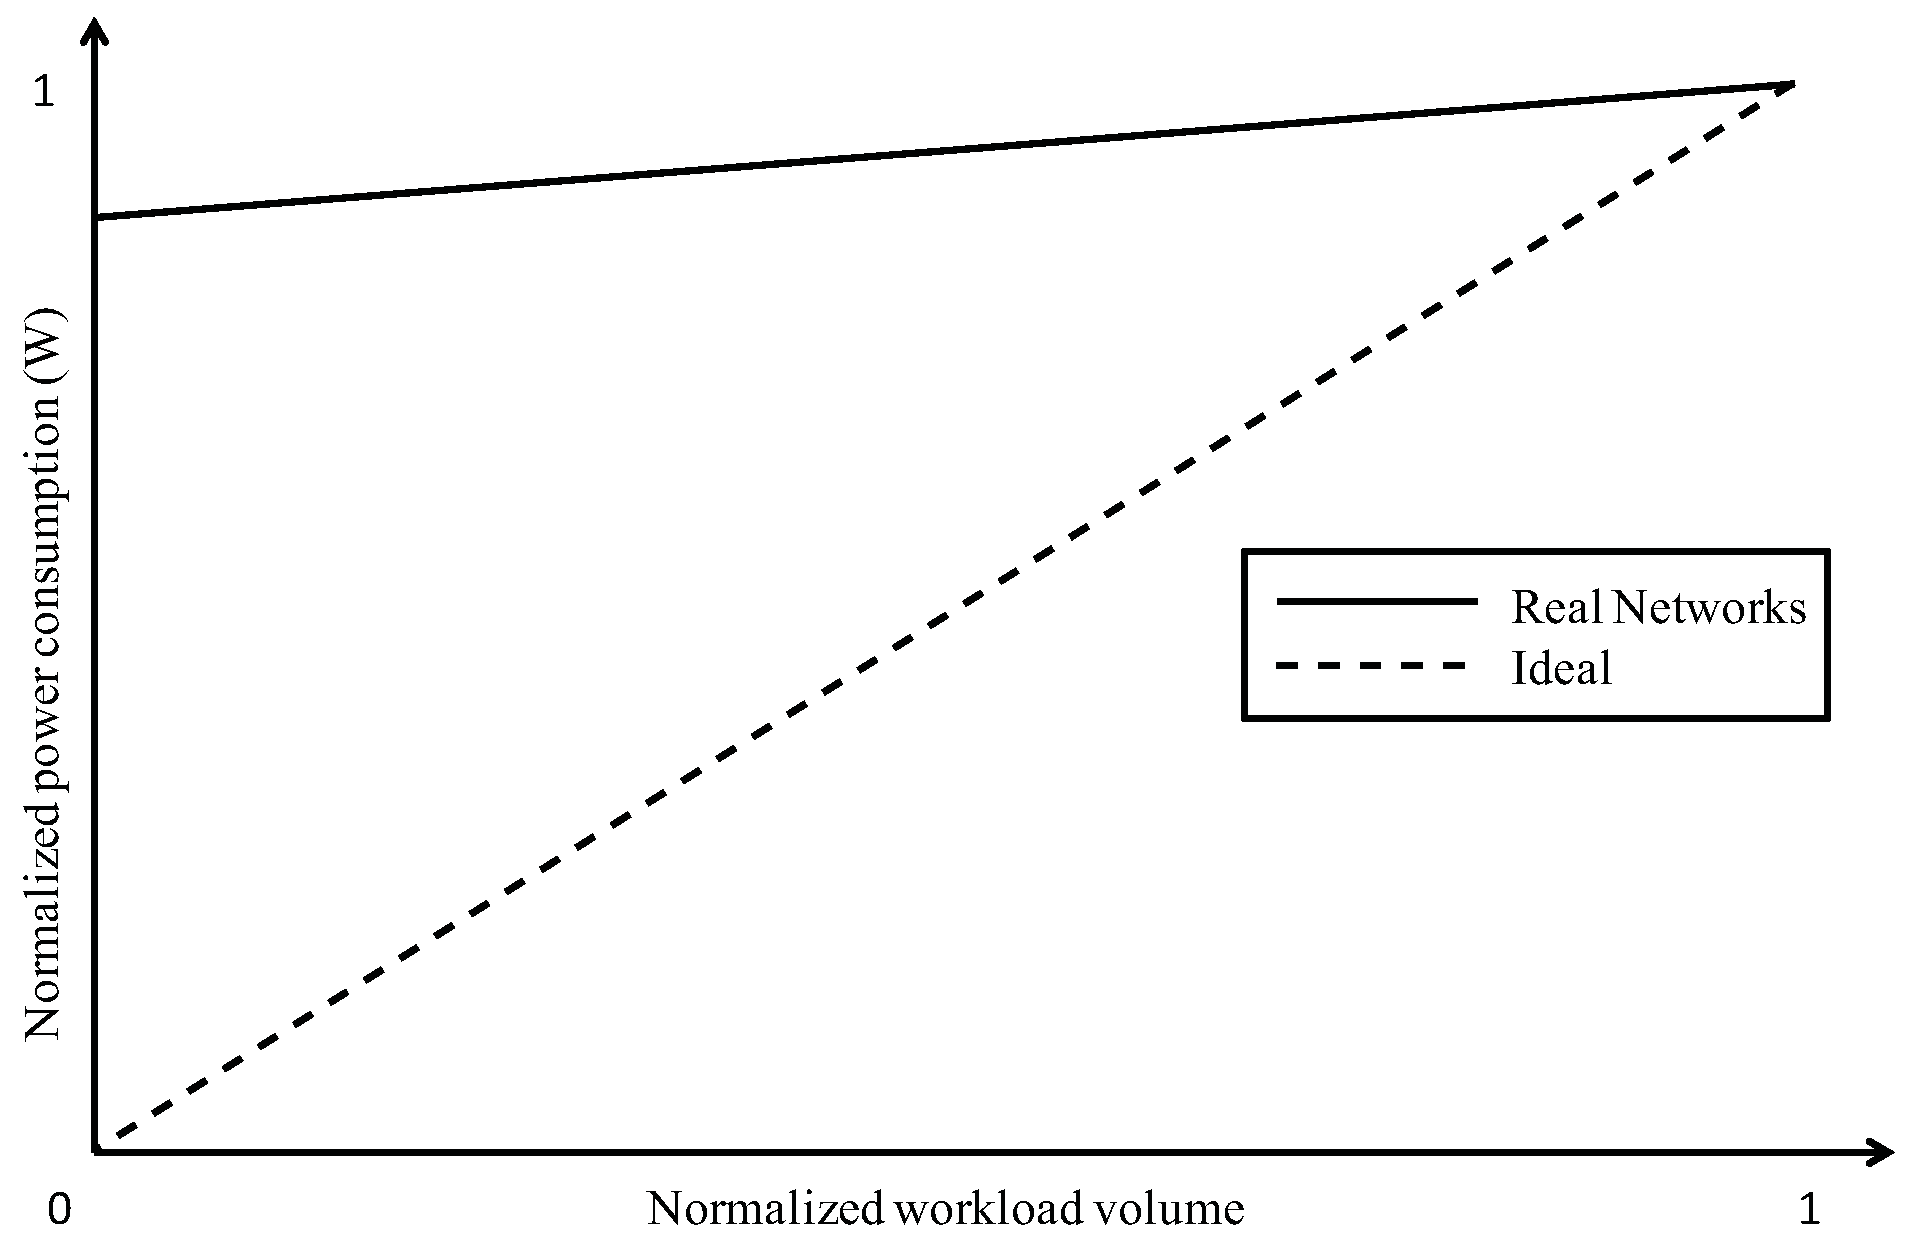
\includegraphics[width=0.7\textwidth]{pics/enerprop.eps}
\caption{Networks lack energy proportionality}
\label{fig:ener-prop}
\end{figure} 

Lack of energy proportionality is of little concern if the network consistently operates in the high workload region because in this region, the power consumption for a real network is close to ideal. However, most networks today have time-varying traffic which is in the low-workload region for considerable amount of time during a given day. Figure~\ref{fig:varwork} shows the workload for call traffic at a cellular site in a large operational GSM network in Pakistan. It shows that call traffic has diurnal cycles and that traffic peaks for only a short period of time during a day. Furthermore, the workload peak is quite high compared to the trough. ISP~\cite{1248656} and data center~\cite{10.1109/MC.2007.443} traffic also show similar trends. 

In order to meet peak expected workload amicably, networks are dimensioned according to the peak workload. Since the workload is far from the peak most of the time and networks are not energy proportional, most networks have a much higher energy consumption than what they would ideally incur. In other words, today's networks are energy inefficient. Another way to look at energy efficiency is through the lens of performance per Watt, a useful metric for energy efficiency of a network. The performance per Watt for today's networks is quite low. Therefore, it is important to lower the y-intercept of the solid line in Figure~\ref{fig:ener-prop} thereby reducing the electricity cost of today's networks without compromising on the performance that they deliver. Recent years have seen significant research focus on improving energy efficiency in both cellular and geo-diverse data center networks.

\begin{figure}
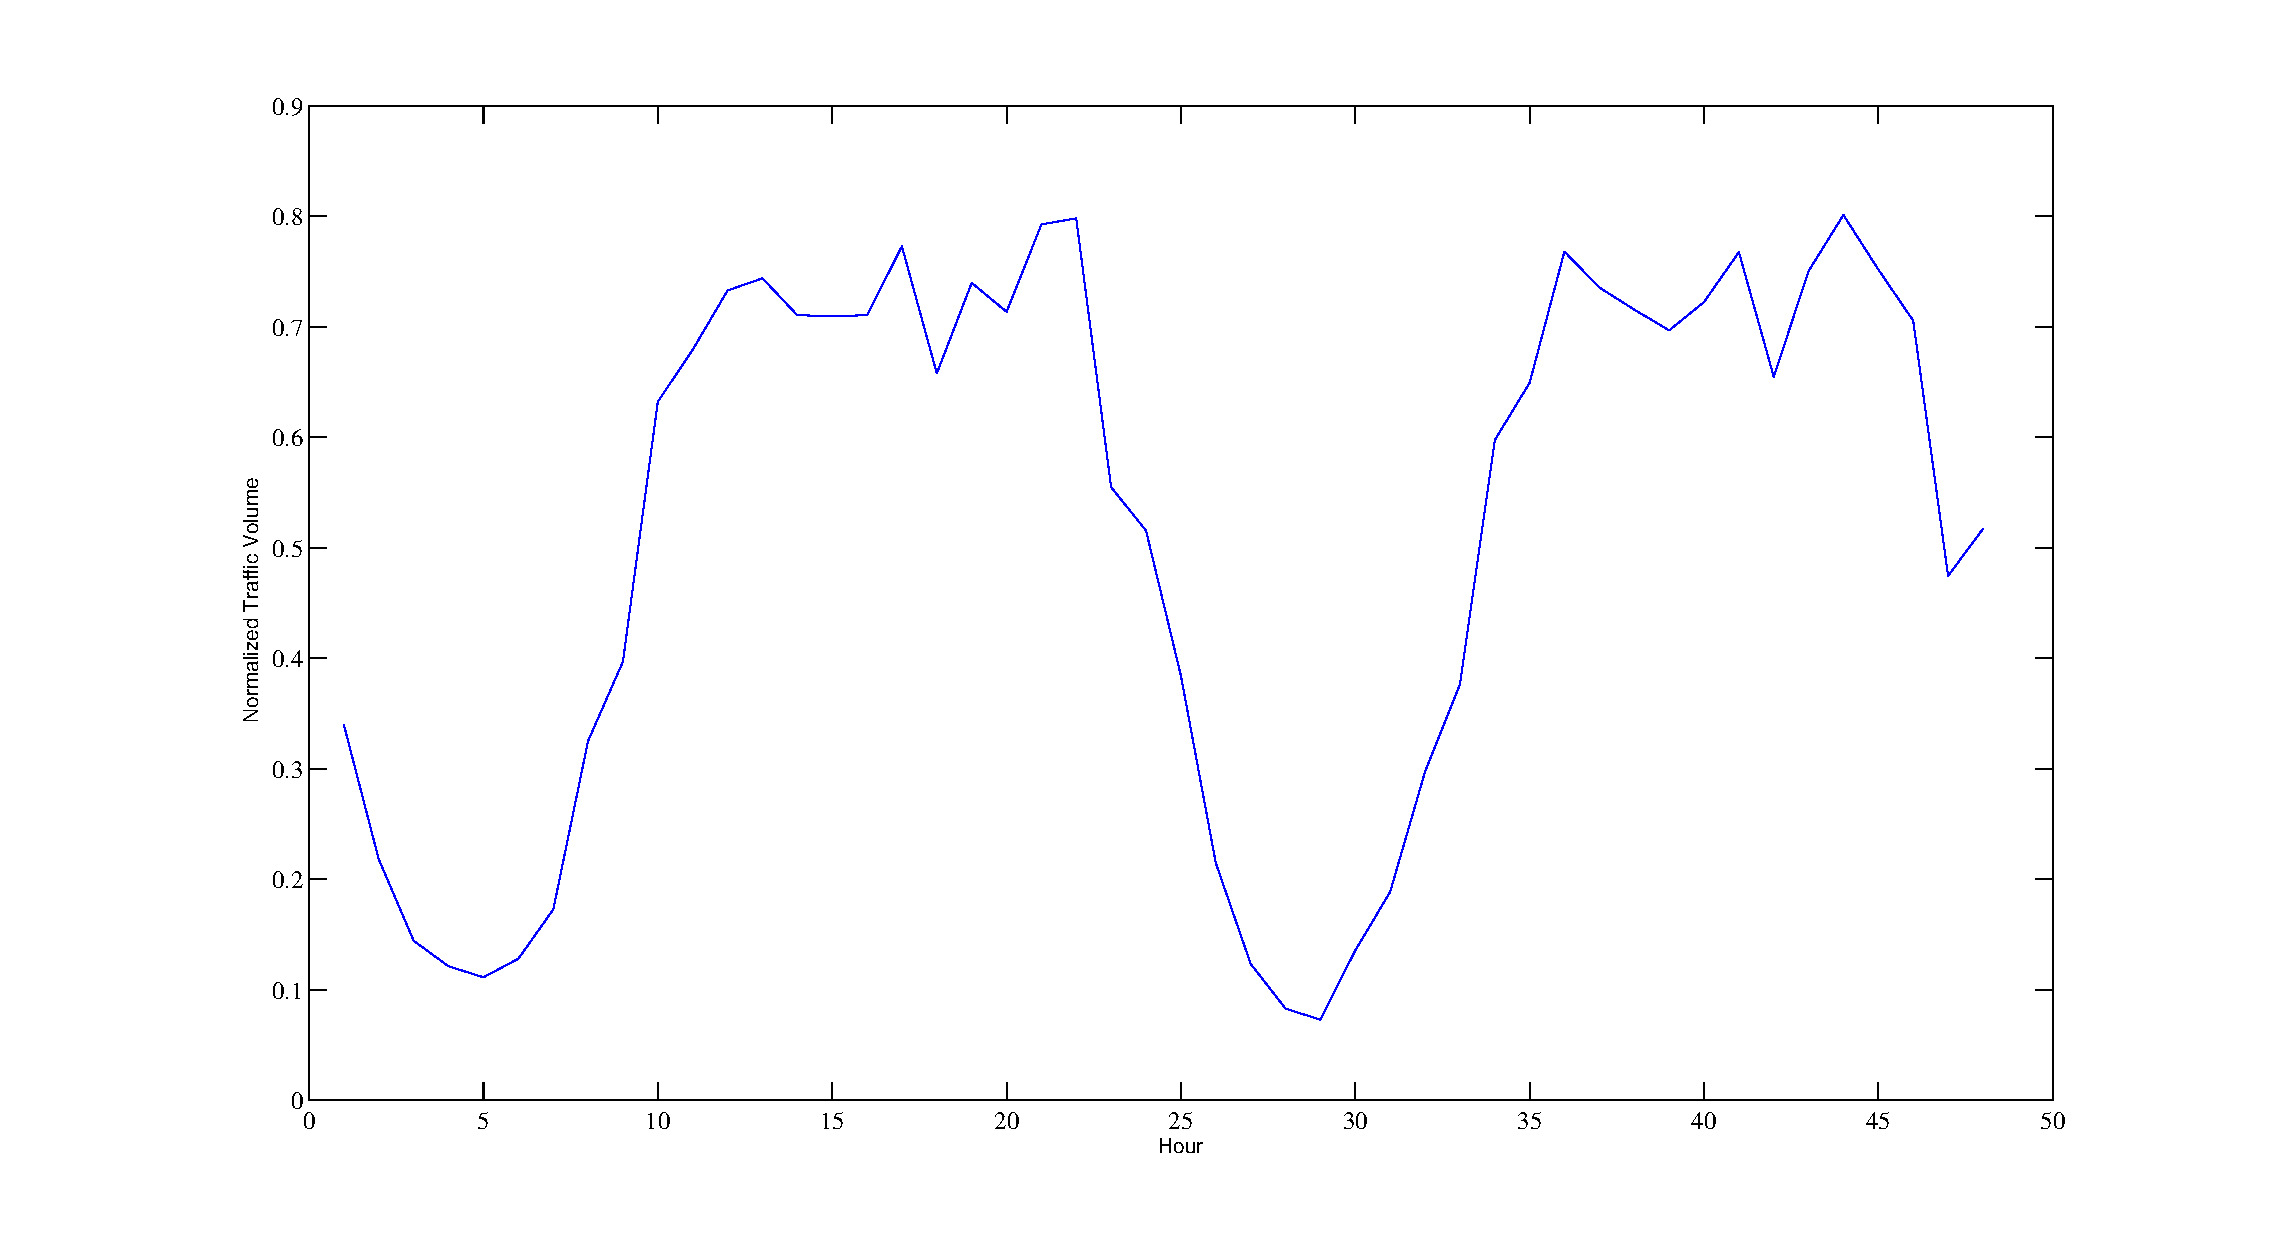
\includegraphics[width=1\textwidth]{pics/waridworkload.eps}
\caption{Call traffic for an oeprational cellular site over two days}
\label{fig:varwork}
\end{figure} 

\section{Prevalent electricity cost reduction techniques} %\textit{Electricity cost} = \textit{amount of energy consumed} $\times$ \textit{unit price of electricity}. Therefore, electricity cost may be cut by reducing either or both of the quantities on the right hand side. 

The electricity cost for a network is given by:
\begin{align}
\text{Electricity cost} = \text{amount of energy consumed} \times \text{unit price of electricity}
\label{eq:elec-cost}
\end{align}
Current work in reducing electricity cost for geo-diverse data centers and mobile cellular networks falls into two categories. The first category focuses on reducing the amount of energy consumed (thereby reducing the first term in equation~\ref{eq:elec-cost}), whereas the second category focuses on using cheaper sources electricity (thereby reducing the second term in equation~\ref{eq:elec-cost}). A taxonomy of the techniques that fall in these two categories is given in the next two sections.

\subsection{Reducing the amount of energy consumed}
\begin{enumerate}
\item \textbf{Hardware upgrades:} Due to ecological challenges, improved energy efficiency is generally a key requirement when developing new technologies and devices. For a given workload demand, an improvement in device energy efficiency lowers the amount of energy consumed, thereby reducing electricity cost. Therefore, hardware upgrades are a way to reduce electricity costs. An operator would, however, opt for hardware upgrades in their network only after they have obtained the Return on Investment (ROI) of the initial deployment or the end of life of deployed equipment. The initial investment not only involves capital cost of equipment but other factors such as spectrum licensing as well. In the cut-throat competition prevalent in most of today's networks, the ROI is slow to achieve. This means that existing energy inefficient networks would stay that way for a considerable time into the future.
\item \textbf{Hardware virtualization:} With the advent of ever faster CPUs, it was observed that servers tend to operate at relatively low CPU utilization most of the time. This was seen as an opportunity to statistically multiplex multiple servers onto a single physical machine by slicing the latter into multiple virtual servers. In this way, virtualization cuts capital costs for procurement of hardware. Since the virtual servers share the same resources (power supply, CPU, network interface, disks), if two servers are multiplexed onto a single physical server, the electricity consumption may be cut by as much as 50\%. A more aggressive server consolidation may cut electricity costs by upto 80\%~\cite{VirtualizationCutsPower}.
\item \textbf{Resource Pruning (RP):} Since network resources must be deployed according to peak demand while the workload peaks only for a short period of time, the excess resource may be deactivated (shutdown or put in power-saving mode depending on what is supported by the equipment) when the workload is low~\cite{Chase:2001:MES:502059.502045,Chen:2008:ESP:1387589.1387613,Meisner:2009:PES:1508244.1508269,Lin_dynamicright-sizing,Peng:2011:TPS:2030613.2030628}. When evaluating the reduction in electricity costs through resource pruning, it is imperative to consider any costs associated with activation and deactivation of network resources.
\end{enumerate}

\subsection{Using cheaper electricity - Workload Relocation (WR)}
Electricity prices exhibit geographic diversity~\cite{qureshiHotnets}, i.e., the price of electricity varies from one location to another. The variation in electricity price is generally noticeable only at large distances. For instance, the electricity price anywhere within a city is generally the same\footnote{With the exception of factors such as different tariffs for domestic, commercial and industrial consumers}. Most networks span large enough distances for geographic diversity in electricity prices to be apparent. 

If the network workload is quite flexible in terms of where it is handled, then the workload originating at a location with high electricity price may be relocated to a different location that has lower electricity price, thereby cutting the cost of electricity. We call this technique Workload Relocation (WR). 

Network workload exhibits varying levels of geo-flexibility. In geo-diverse data centers, for instance, the workload is highly geo-flexible, i.e., a client's request may be handled close by or even hundreds of miles away. On the other hand, the workload in cellular networks has very low geo-flexibility, i.e., a call must be handled at a cellular base station within a few hundred meters from the caller. Therefore, the amount of electricity cost savings achievable by exploiting geo-diversity in electricity prices through the use of WR is expected to be higher in data center networks than in cellular networks.

Electricity prices also exhibit temporal diversity~\cite{qureshiHotnets}, i.e., the relative order of electricity prices at different locations keeps changing. If a city in Kansas presently has chepaer electricity than one in Oklahoma, an hour later, the reverse may be true. This means that mapping of workload to locations must be periodically updated. The granularity of these updates depends on how frequently electricity prices change. Deregulated electricity markets, such as the ones in the USA, exhibit price changes at two different time scales (15 minutes for real-time electricity prices and an hour for day-ahead prices). 


\section{Our thesis} Based on the similarity in workload characteristics and the dependence of power consumption on workload, we opine that a generalized power optimization framework may be formulated that is applicable to many different types of networks. In this thesis, we focus specifically on geo-diverse data center networks and cellular networks. Our generalized electricity cost optimization framework would use workload relocation and resource pruning in tandem to reduce electricity costs\footnote{Hardware virtualization is complimentary to our framework}. 

\section{Contributions} This thesis makes the following contributions:

\begin{itemize}
\item We present a generalized model for electricity cost optimization applicable to different types of networks that jointly uses workload relocation and resource pruning. We show that this problem is NP-Hard.
\item We present a framework called Relocate Energy Demand to Better Locations (RED-BL), pronounced Red Bull, that solves the electricity cost minimization problem. We apply RED-BL to geo-diverse data centers as well as cellular networks using real data traces.
\item We obtain optimal solutions to RED-BL problems for both data center and cellular networks for realistic problem sizes. To handle the intractability of the problem, we also propose some heuristics that would be useful for even larger instances of the electricity cost minimization problem. 
\item Prior efforts in this area had mostly ignored the costs associated with activation and deactivation of network resources. To the best of our knowledge, we are the first to incorporate these in our optimization framework.
\item A network with significant over-provisioning may handle most of the workload at cheaper locations while the more expensive locations may be temporarily pruned from the network. In other words, geographic diversity in electricity prices incentivises over-provisioning. We study the benefits of increased over-provisioning and find diminishing returns with over-provisioning.
\end{itemize}

\section{Organization} The rest of the document is structured as follows. In Chapter~\ref{chap:background}, we compare two different types of networks and describe how similar they are in terms of workload handling and power consumption. In chapter~\ref{chap:framework}, we derive a generalized power consumption model, applicable to different types of networks and formulate RED-BL, a generalized electricity cost optimization problem. We present an evaluation of RED-BL on geo-diverse data centers and cellular networks in chapters~\ref{chap:casestudy1} and~\ref{chap:casestudy2}, respectively. In chapter~\ref{chap:conclusions}, we draw the conclusions and provide additional future directions.
\chapter{Background - Power consumption models in geo-diverse data centers and cellular networks}
\label{chap:background}
In this chapter, we first describe the power consumption models for geo-diverse data centers and mobile cellular networks. Then, we draw similarities between these two networks to come up with an abstract power consumption model. This generalized power consumption model motivates the formulation of a generalized electricity cost optimization framework in the next chapter. 

\section{Geo-Diverse Data Centers - enablers of cloud computing} Traditionally, an individual or organizations that requires computing resources would procure it. Authors needing to do electronically typeset manuscripts from home would buy a PC with word-processing software. Organizations that need to deploy an Enterprise Resource Planning (ERP) system would buy servers and install the required software on these. This involves upfront expenditure on equipment and software licensing costs as well as recurring expenses resulting from factors such as renewal of software licenses, salaries for staff to smoothly run the software and training to customize and operate the newly acquired software. On the other hand, we use utilities such as electricity, water, telephone and gas without having to deploy and run facilities power generation plants or water storage systems. We just pay a per-use subscription charge to some organization that does it for us, while we just consume the utility as needed. Due to economies of scale, utilities are economical for the end user. It was envisioned that computing could also be offered as a utility, to be consumed and sometimes paid for, as needed. This is the vision of cloud computing.

Based on the flexibility and sophistication of the service being offered, cloud computing has various service models, as described below: 

\begin{itemize}
\item \textbf{Infrastructure as a Service (IaaS)}: In this model, the consumer gets access to one or more servers hosted and managed by the service provider. The consumer is responsible for installing the Operating System (OS) and any other software according to their requirements. Amongst all cloud computing models, this one offers the greatest flexibility to the end user. The end user can choose which Operating System they want to run. They can deploy their own customized applications on the server. This also means that the great responsibility of server software management lies on the end user. Amazon Web Services (AWS), Microsoft Azure and Google Compute Engine are examples of IaaS.
\item \textbf{Platform as a Service (PaaS)}: In this model, the service provider offers a complete computing platform with a pre-installed Operating System (OS). The computing platform generally also includes other pre-installed software such as a database management system (DBMS) and programming environment. The service consumer can deploy their required applications on the platform as long as it meets the application's software requirements. Microsoft Azure offers PaaS model services.
\item \textbf{Software as a Service (SaaS)}: A service user often wishes to be least concerned with software installation, configuration and maintenance. The cloud computing model for such cases is SaaS. Web-based email services such as GMail are a common example of SaaS.
\end{itemize}

In order to offer cloud computing, cloud operators deploy large facilities called data centers. A given data center may have tens of thousands of servers to provide computing as a utility. Cloud operators typically deploy multiple data centers at different geographic locations. This is done for two reasons. First, having data centers at different locations provides fault tolerance. If one site goes down for some reason, the other site may take over as a backup. Also, multiple remote sites are less likely to be affected simultaneously by a natural disaster. A second reason to have multiple data centers is to have low latency to clients at different locations. For instance, Amazon has multiple data centers in different continents, thereby ascertaining that no matter where a client may be, there is an Amazon data center relatively close by compared to the case if Amazon only had one data center in the US. Figure~\ref{fig:googledcmap} shows the locations of Google's data centers across the globe (according to www.google.com/about/datacenters/inside/locations/ as of August 10, 2014).

\begin{figure}
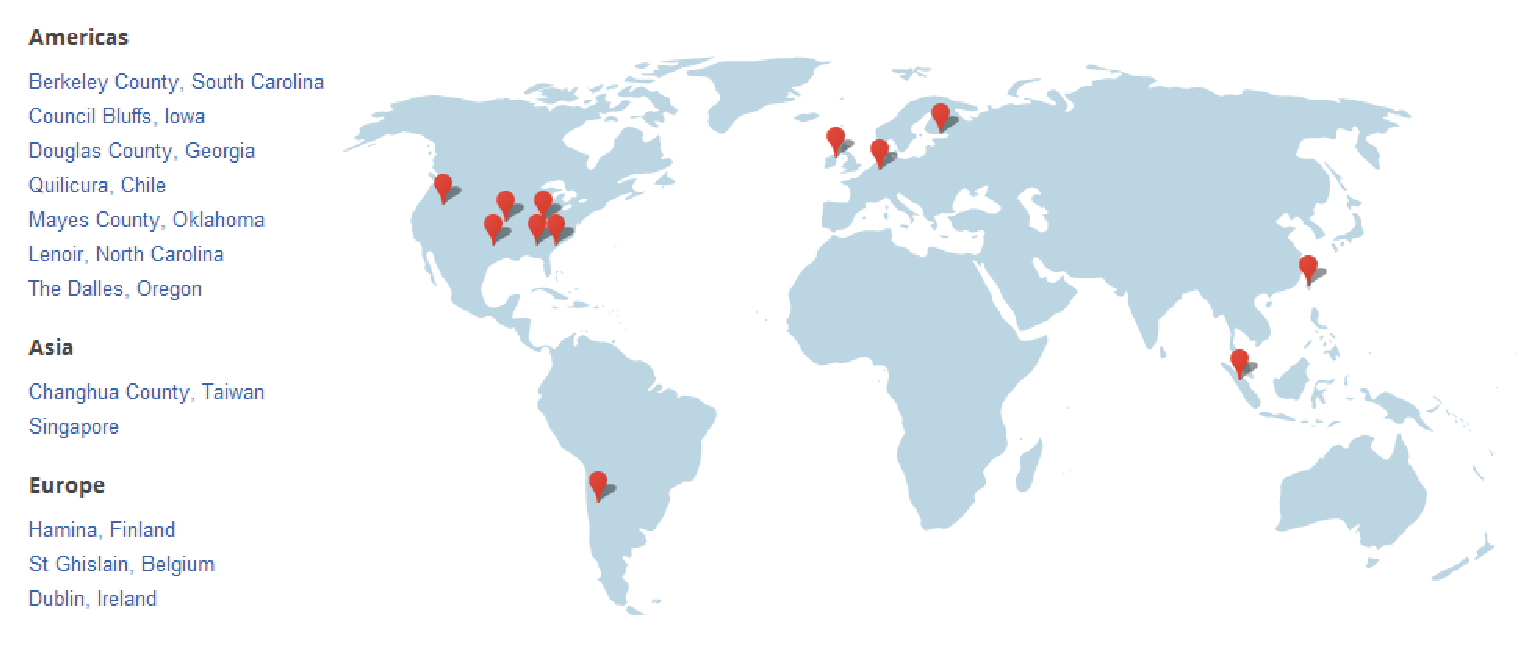
\includegraphics[width=1\textwidth]{pics/googledcmap2.eps}
\label{fig:googledcmap}
\caption{Google Data Center Locations - Source: www.google.com/about/datacenters/inside/locations/}
\end{figure}

\subsection{Structure of a data center} Today's data centers are organized hierarchically~\cite{dcnetworking:vahdat:micro:2010}, as shown in Figure~\ref{fig:dcheir}. A typical data center hosts tens of thousands of servers~\cite{Abts:2012:GTD:2184319.2184335}. The servers are installed in vertical racks. Apart from servers, the racks host other equipment as well. In addition to built-in hard drives in the servers, some dedicated storage nodes are also installed in the racks. A high speed Ethernet switch provides interconnection between the devices installed in the rack and connectivity to the rest of the data center and beyond. Power supply and distribution units for the equipment are also installed in the rack. 

A group of racks, called a pod (or a cluster), are interconnected by means of aggregation switches. An aggregation switch allows servers in different racks to communicate with each other. All the pods within a data center are interconnected by core switches. This allows servers in different pods to communicate with each other. The core switches are interconnected through one or more border routers. These border routers are the avenues for traffic coming in and going out of the data center. 

\begin{figure}
\includegraphics[width=1\textwidth]{pics/dcheir.eps}
\caption{The modern data center's architecture}
\label{fig:dcheir}
\end{figure}

All of the equipment is quite tightly packed within a pretty small space in a data center. The equipment generates a lot of heat and to prevent thermal damage to it, cooling must be provided. This is generally done by air-cooling, i.e., heat is transported away from the equipment by circulating cool air around it.

\subsection{Inter-data center traffic} An operator typically deploys multiple data centers that are geographically distributed. Each of these data centers is inter-connected by means of high-speed inter data center network links. These links serve to carry various types of traffic, some of which are given below:
\begin{itemize}
\item \textbf{Consistency traffic:} An operator often maintains replicas of some of the servers in their data centers. These replicas are maintained for achieving one or both of the following three objectives: high throughput, resilience and low-latency to clients. Multiple replicas that handle client requests simultaneously can help to increase the effective throughput, i.e., the number of requests handled per second. Sometimes a replica does not actively handle client requests until the primary server fails. When such an event occurs, the replica takes over and offers continued services to the clients. Lastly, by geographically distributing several replicas of a server and routing client requests to the nearest replica, the client latency to the server can be minimized. 

Unless the content being hosted by a server is static, which is rarely the case these days, replication incurs an overhead. Whenever content on one server changes, the change must be reflected to all other replicas. For instance, a customer's website may be hosted at two different data centers and whenever a change is made to one copy of the website, the same changes must be reflected at the replica as well. This action requires network traffic between the data centers that host the replicas. 
\item \textbf{Background traffic due to load-balancing:} Some traffic on the inter-data center links may be a result of the effort to achieve load-balancing amongst the data centers. As an example, consider a web-based email service provider that has partitioned user inboxes over the data centers. One objective of this partitioning may be that roughly the same amount of storage space is used at each data center. Since user inbox sizes are not static (growing when new emails are received and shrinking when emails are deleted) and these inboxes may grow and shrink at different rates, depending on factors such as number of mailing lists that a user subscribes, the partitioning of users amongst data centers must be dynamic as well. The operator must periodically determine a new user partitioning that results in roughly equal storage space being consumed at each data center. In order to achieve this balanced storage size, some users' inboxes must be moved from one data center to another, over the inter-data center links.
\item \textbf{Background traffic due to distributed computing:} Handling client requests in a distributed fashion requires network traffic overhead due to different servers communicating requests, intermediate results and final responses. For instance, a web search provider may distributed the web's index over multiple data centers. When a search query is being processed, the request must be sent to all data centers over the inter-data center links and the responses from the data centers must be aggregated after being be received on the same links.
\end{itemize}

\subsection{Handling of client requests} 
%front-end server based load balancing and request routing mechanisms such as IP Anycast
We observed in chapter~\ref{chap:intro} that electricity cost depends not only on how much workload is handled, but also where it is handled. Thus, in order to develop a model for electricity cost in a geo-diverse data center, we need to first understand how workload from all over the globe is distributed amongst the data centers. In this section, we will use as an example a client request for viewing a web page hosted by a geo-diverse data center operator. 

To access a web resource, the user types a uniform resource locator (URL) in the web browser's address bar. The URL typically contains the Fully Qualified Domain Name (FQDN), such as www.google.com, corresponding to the web server that hosts the requested resource\footnote{It is also possible to specify the IP address of the web server directly in the URL.}. Since a single server would hardly be sufficient to handle all traffic for a popular web site, several servers must be mapped to the same FQDN. However, the web browser must connect to exactly one of these servers to fetch a particular web resource. Figure~\ref{fig:dcloadbalance} briefly describes how this web server's IP address is picked. For details on DNS resolution process, see~\cite{rfc1034,rfc1035}. 

\begin{figure}
\centering
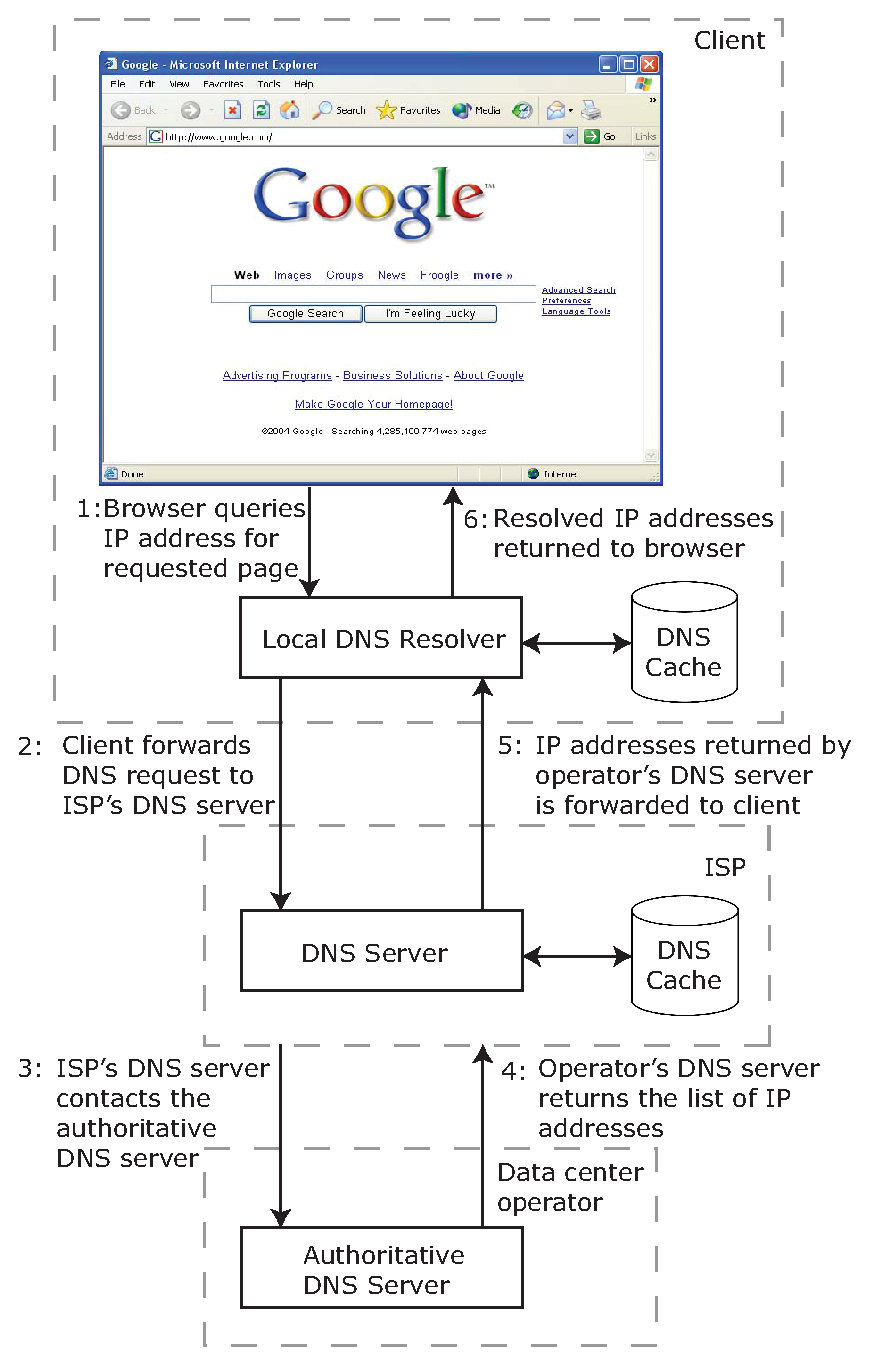
\includegraphics[width=0.5\textwidth]{pics/dcloadbalance.eps}
\caption{Resolving the IP address for a server hosted in a data center}
\label{fig:dcloadbalance}
\end{figure}

When the user directs the web browser to fetch a web page by typing a URL in the address bar, the browser invokes the local Domain Name System (DNS) resolver on the client machine which attempts to determine the IP address corresponding to the DNS name of the remote host specified in the URL. The local DNS resolver communicates with the DNS server for the client's ISP\footnote{Some people configure other DNS servers, such as Google's Open DNS Servers on their machines. In such cases, the local DNS resolver would communicate with those other DNS servers.}. The DNS query eventually reaches the authoritative server for the remote host's domain. In our example, this would be operated by the data center operator. The DNS server for the data center operator resolves the DNS name by returning a list of IP addresses corresponding to the servers that are associated with the DNS name specified by the client. When the client receives the DNS response containing list of IP addresses, it picks one of the IP addresses to fetch the web page. For simplicity, many web browsers simply pick the first IP address in the list. If, for some reason, the web browser is unable to connect to that IP address, it tries the second one on the list and so on. For consecutive responses to DNS queries for the same FQDN, DNS servers often rotate the list of IP addresses in each response so that if the client simply picks the first IP address, the servers are likely to receive equal workload.

Notice in Figure~\ref{fig:dcloadbalance} that caches are available at various DNS resolvers in order to improve the latency of DNS resolution. These caches will keep the list of IP addresses corresponding to recently queried DNS names until the timeout specified by the authoritative DNS server occurs.

The data center operator has a large pool of IP addresses (IP address space) for their layer 3 devices. This IP address space is segmented over the geo-distributed data centers. The IP address picked by the client from amongst the list received from the operator's DNS server belongs to one of these data centers. The client must now send its Hyper Text Transfer Protocol (HTTP)~\cite{rfc1945} request to the server corresponding to the chosen IP address. To this end, the client establishes a Transport Control Protocol (TCP) connection with the server using the selected IP address. An HTTP request is sent over this TCP connection and a response is received. During this communication, packets from the client leave the client's network interface and are routed by the ISP until they reach the data center where the required web server is hosted. The border router in the data center forwards these packets to the server with the destination IP address. En-route, these packets traverse the core, aggregation and top of rack switches. The response packets are forwarded from the web server back to the border router which routes it back to the client machine.

\subsection{Data center power consumption model} 
%Describe the power consumption model from prior work and derive a more simplified yet equivalent model
The electric load within a data center may be categorized into (i) IT load and (ii) non-IT load. The IT load includes servers, network equipment and network storage. The non-IT load includes power supplies, un-interruptible power supplies (UPS), air-conditioning and lighting. 

Fan et. al. used the results of a measurement study to show that the total power consumption in a data center can be well-modeled as an affine function of the average CPU utilization~\cite{Fan:power:ICSA:2007}. As more and more client traffic arrives at servers in a data center, the average CPU utilization increases. Therefore, data center power consumption can also be represented as an affine function of workload. 

\section{Cellular Networks} %Just as data centers enable applications that we rely on every day, cellular networks are an important enabler of another pervasive service: telephony.
Mobile telephone systems have enabled not only untethered access to traditional telephony services but also new types of services. We make phone calls, send text messages and can even connect to the Internet using our mobile phones. Just as Internet connectivity services are provided by ISPs and Internet applications are powered by data center operators, mobile phone services are provided by mobile network operators (MNOs).  

Over the years, mobile networks have been deployed based on different technologies. Literature often categorizes mobile network technologies in terms of \textit{generations}. First generation cellular networks (1G) were based on Advanced Mobile Phone System (AMPS). AMPS networks were deployed starting in 1978. The AMPS system also evolved into Digital-AMPS (D-AMPS) networks. Two technologies were part of the second generation (2G) cellular networks, namely Global System for Mobile communication (GSM) and Code Division Multiple Access (CDMA). Anticipating the increased demand for mobile access to data services such as Internet access, vendors introduced General Packet Radio Service (GPRS) as an add-on to GSM networks. GPRS offers data rates between 56 kbps and 114 kbps. A GSM network with GPRS is sometimes referred to as 2.5G. GPRS bit rates are insufficient for many high bandwidth applications such as video calls, video streaming and video conferencing. To enable such services, broadband mobile services were introduced in third generation (3G) networks networks such as High Speed Downlink Packet Access (HSDPA) and Universal Mobile Telephone System (UMTS). The increasing trends in the use of high-bandwidth applications in mobile networks has spawned the fourth generation (4G) cellular networks such as Mobile WiMAX and Long Term Evolution (LTE). In this thesis, we consider only GSM cellular networks.

\subsection{Structure of a cellular network} %A really basic introduction to cellular networks covering: concept of cells, mobile stations (MSs), Base Transceiver Stations (BTSs) and Base Station Controllers (BSCs)
Mobile phone networks are also referred to as cellular networks because the area covered by the operator is logically divided into several small areas called cells. A cell in an urban setting (a macrocell) is typically upto a few hundred meters in radius, whereas in suburban or rural settings, the cell radius may be as large as a few kilometers. A \textit{cell site}, typically situated in the middle of a cell, enables subscribers in that cell to connect to the mobile network. A cell site, often referred to as a Base Transceiver Station (BTS)\footnote{A single cell site sometimes hosts multiple BTSs, for instance, when multiple network operators share a single site} or simply a base station, hosts a number of transceivers (TRXs), radio antennas, power amplifiers and other allied equipment. 

A cell is typically divided into three sectors, resembling 120 degree pie-slices, each covered by different directional antennae. Each sector may have multiple TRXs. A typical cell configuration is one with six TRXs in each cell, referred to as a 6+6+6 cell. 

GSM uses a combination of frequency division multiple access (FDMA) and time division multiple access (TDMA). Multiple frequency channels are available in each sector - one for each TRX - and each frequency is divided into eight time slots. A particular frequency and a particular time slot identify a physical channel. A few physical channels in each sector are reserved for control signaling purposes and the rest can be used for user traffic such as voice calls. Since the number of physical channels represents traffic capacity, and the number of physical channels is proportional to the number of TRXs in a sector, the number of TRXs represents a cell's traffic capacity.

The duration of each time slot for a given frequency is 0.577 ms. A group of eight time slots for a given frequency is collectively referred to as a GSM frame. The transmission in each time slot for a given frequency is termed as a burst. The recurrence of a particular burst across all GSM frames is a physical channel. A group of 26 GSM frames is referred to as a GSM multi-frame.

A government regulator such as Pakistan Telecommunication Authority (PTA) allocates a frequency band to each of the operators providing cellular service in the host country. This band The allocation is such that each operator gets a different frequency band. The operator distributes their allocated band to cells in their network. The channels allocated to an operator are much fewer than the number of cells in the network. Therefore, a given channel must be reused in an operator's network. Frequency reuse is done in such a way that any two cells that share the same frequency channel are sufficiently far apart so that the radio signal from any one of the cells does not noticeably interfere with that in the other. In fact, each cell is typically divided into three sectors (resembling 120 degree pie-slices), therefore, the frequency allocation is done on a per-sector basis. Nonetheless, for a high-level view, the set of frequencies allotted to all sectors in a cell can be considered as allotted to the cell itself. Each TRX at a cell site operates at a distinct frequency\footnote{Given two communicating parties at fixed locations, if the transmitted signal power is kept constant, the received radio signal strength would differ depending on the frequency used. Also, this frequency selective behavior of the radio communication medium keeps changing with time, i.e., if frequency A receives better propagation compared to frequency B at time $t_1$, the same will not necessarily be true at time $t_1+\epsilon$. This means that we can't statically pick the best frequencies to use for a particular cell by considering, for instance, the type of terrain. In order to make decent communication conditions available to all callers, on average, GSM networks also use frequency hopping, whereby the frequency allocation to cells are changed periodically.}. 

Frequency assignment and frequency hopping are examples of activities that require coordination. For systematic coordination of radio resources, Base Station Controllers (BSCs) are deployed in the network. The operator's coverage area is geographically split into zones, each of which is controlled by a single BSC. The BTSs communicate with the BSC via backhauls such as E-1 links or microwave. Since a BSC only controls a subset of BTSs, it can only perform local coordination. In order to ensure global coordination in radio resource allocation and control, the BSCs are also interconnected using backhaul links.

A mobile station (MS) often receives radio signals from multiple BTSs nearby. The MS picks the BTS from which it receives the strongest signal as its serving BTS. A MS will do all communication such as call reception and placement through the serving BTS. When a subscriber moves around in the operator's coverage area, the signal from the serving BTS might weaken. In such an event, the MS requests the network to allow it to change the serving BTS to the one from which it currently receives the strongest signal. This call handoff is coordinated by a Base Station Controller (BSC). 

Another key component of a GSM network is the Mobile Switching Center (MSC) that is responsible for call routing both within the GSM network and beyond (to a landline phone, for instance). Since the focus of our thesis is power consumption in the network and 50\%~\cite{Louhi:2007:BTSPower:INTELEC} - 80\%~\cite{Oh:Comm:2011} of a cellular netowrk's electricity consumption is due to the BTSs, we will not dwell on the MSC and other components of the cellular network any more than necessary.

\subsection{Call placement} %How a call is handled by a BTS (at a very abstract level, i.e., how is the serving BTS chosen). Role of the BSC in cell association and call hand-off
To place a voice call, when a user enters the phone number digits on the MS and presses the send button, the MS requests the BTS to acquire a channel to communicate with the MSC. Once this channel is successfully acquired, the MSC authenticates the MS, sets up encryption so that the call data is secure. The MS then send the dialed digits to the MSC. The MSC instructs the BSC and MS to switch from signaling mode to voice mode and attempts to route the call to the called numbers. A downlink channel is assigned so that the ringing tone and called party voice can be heard on the calling MS. If there is an error in call establishment, an error message is heard on the calling MS over the same channel. In short, two channels are required to support a voice call in the sector where the call originates.

A sector with $n$ TRXs has $8n$ physical channels. It appears that the sector should be able to support $4n$ calls because each call requires two physical channels. However, the actual maximum number of simultaneous calls is different from this number for two reasons: 
\begin{itemize}
\item Some channels are reserved for control purposes, the exact number of such channels varies from operator to operator.
\item GSM supports two different types of codecs, namely the full-rate codec and the half-rate codec. The full-rate codec corresponds to a caller using a burst in every GSM frame during a call, whereas the half-rate codec corresponds to a caller using a burst in every alternate GSM frame. By default, the full-rate codec is used for every call. However, when traffic congestion rises above an operator-configured threshold, the network attempts to admit every new call using a half-rate codec, if the corresponding MS supports it. If the traffic rises further and crosses a second threshold as configured by the operator, the network also re-assigns current calls to use a half-rate codec depending on the corresponding MS support. This enables a BTS to support more than $8n$ simultaneous calls during times of congestion.
\end{itemize}
 

\subsection{BTS power consumption model} %Describe the power consumption model from prior work
BTSs account for most of the power consumed in a cellular network. Louhi~\cite{Louhi:2007:BTSPower:INTELEC} claimed that BTSs contribute 50\% of overall network power consumption, whereas Oh et. al~\cite{Oh:Comm:2011} put this number at 80\%. For this reason, most of the prior work related to power consumption in cellular networks focuses on BTSs. 

Lorincz et. al. performed a measurement study of BTS power consumption under real-traffic conditions. They concluded that the BTS power consumption may be approximated as an affine function of call traffic~\cite{Lorincz:BTS-Measure:Sensors:2012}. Thus, as traffic varies during a given day, instantaneous power consumption would follow a similar curve as the traffic. 

\section{A comparison of data center and cellular networks} %Geo-diverse data centers and cellular networks are similar in the sense that both are built out of network resources to handle workload which results in electricity consumption. 

\begin{table}
\begin{center}
\begin{tabular}{|c|c|c|}
\hline \ & Geo-diverse data centers & GSM cellular networks \\
\hline Traffic Characteristics & Diurnal patterns & Diurnal patterns \\
\hline Network capacity & Dimensioned according & Dimensioned according \\
\ & to peak workload & to peak workload \\
\hline Energy proportionality & No & No \\
\hline Power consumption & Affine function of workload & Affine function of workload \\
\hline Geo-diversity in & Yes & Limited \\
electricity prices & \ & \ \\
\hline Geo-flexibility in & \ & \ \\
resource selected for & High & Low \\
workload handling & \ & \ \\
\hline
\end{tabular}
\caption{A comparison of data center and cellular networks}
\label{tab:contrast}
\end{center}
\end{table}

From our discussion of geo-diverse data centers and cellular networks, we note that these networks have several similarities and some subtle differences apropos their power consumption. Keeping their similarities and differences in mind, abstractions can be identified to generically represent these networks. These similarities and differences are summarized in Table~\ref{tab:contrast}. Both of these networks are a collection of resources that handle workload. The resources are servers and TRXs in case of data centers and cellular networks, respectively. The workload is clients' computing requests such as web page views in case of data centers, whereas it is voice calls in case of cellular networks. The workload in both types of networks exhibits diurnal patterns~\cite{10.1109/MC.2007.443,Peng:2011:TPS:2030613.2030628}. The network in both cases is provisioned according to peak workload demand. Since the network resources are not energy proportional, this means that in low-workload regimes, the network is heavily over-provisioned. Thus, both of these networks are energy inefficient. The power consumption for both networks is an affine function of the workload. 

A subtle difference between geo-diverse data centers and cellular networks is that the former is characterized by geo-temporal diversity in electricity prices. Furthermore, any client request may be handled at any data center, irrespective of their location. Thus, for a given client request at a given time, the candidate servers are deployed in data centers situated at locations with different electricity prices. In case of cellular networks, however, a given call may be handled at only a few BTSs in the vicinity, which are so close that an electricity price differential is unlikely. 

\section{Discussion}
In this chapter, we have seen that there are certain similarities between geo-diverse data centers and cellular networks apropos their power consumption. We have used these similarities to identify abstractions for a general model of these networks in terms of their power consumption. In the next chapter, we will use these abstractions to derive such a generic power consumption model and thus, formulate an electricity cost minimization framework.
\chapter{A generalized framework for electricity cost optimization}
\label{chap:framework} In the last chapter, we have seen that networks, such as geo-diverse data centers and cellular networks, are energy inefficient. This is due to lack of energy proportionality coupled with significant variations in workload. We have also observed that these networks are plagued by high electricity costs. For a given electricity price, if these networks were energy efficient, high electricity costs would only be due to heavy workload. However, energy inefficient networks consume a lot more energy than they ideally should. Hence, high network electricity costs are a source of concern. 

One way to deal with this energy inefficiency is what we call resource pruning (RP). The idea is to deactivate some network resources when they are not needed. Since the workload is variable, the operator must periodically determine the optimal network configuration, i.e., the active/inactive state of each network resource and the mapping of each unit of workload to 

\section{Modeling the electricity cost minimization problem in networks and systems} Discuss how different network types can periodically use RP and WR to minimize electricity costs. Show that this problem is NP-Hard. Describe the concept of network state and motivate a state trajectory optimization problem. Describe transition costs and formulate a mathematical optimization problem. 
\subsection{The objective function} Provide the mathematical form of the objective function that is designed to solve the optimal state trajectory problem.
\subsection{The constraints} Comment on some of the network-specific constraints that the optimization must be subject to.


\chapter{Case Study I: Geo-diverse Data Centers}
\label{chap:casestudy1}
\section{Prelude}
Geo-diverse data centers enable robust and low-latency cloud services. The electricity cost for this huge infrastructure is a significant fraction of the operational cost (15\%)~\cite{costCloud} as well as capital cost~\cite{qureshiHotnets}. Due to increasing demand for cloud services and increasing electricity prices, it is essential for data center operators to cut their electricity bill~\cite{brill:DataCenterCrisis:UI:2007,Belady_EC_2007}.

In the previous chapter we presented an abstract and generalized electricity cost minimization framework that is applicable to geo-diverse data centers as well as cellular networks. In this chapter, we will derive a specialized instance of the general problem, discuss it's solution (exact as well as heuristic) and perform a sensitivity analysis.  We will also discuss our formulation's benefits and limitations.

The electricity cost savings resulting from workload relocation are somewhat limited due to lack of energy proportionality in today's data centers~\cite{10.1109/MC.2007.443}. Therefore, it was proposed to dynamically scale the active infrastructure in response to temporal variations in workload~\cite{10.1109/MC.2007.443,qureshi2009cutting}. This capacity scaling is expected to incur some overhead electricity cost which may be modeled as the \textit{state transition cost} in the state trajectory problem. 

Theoretically, one can benefit from capacity scaling by shutting down some equipment when it is not needed. However, some equipment in data centers may not be shut down because it is critical in nature. We term such equipment as inelastic load and the rest of the equipment as elastic load. Resource pruning of elastic load in data centers minimizes the electricity consumption, but conventional wisdom suggests that restarts affect equipment lifetime and operators are generally reluctant to adopt this approach. On the other extreme, elastic load may be left in an idle state, but the reduction in electricity  consumption would be quite small. In between these two extremes would be Dynamic Voltage and Frequency Scaling (DVFS) techniques. The transition cost would be zero for the idling scheme since no state-change overhead is incurred. The transition costs would be quite high if elastic load is de-activated (and activated later when needed), whereas DVFS would account for transition costs somewhere between the two extremes~\cite{Meisner:2009:PES:1508244.1508269}. In this thesis, we experiment with the entire spectrum of transition costs in order to generalize our results.

%The electricity load at a data center may be partitioned into two sets: one that is inelastic and must be on all the time and the other elastic portion that may be shutdown if there is no workload for the data center to handle. Let the first set comprise a fraction $r$ of the total data center power draw. The second part accordingly contributes a fraction $(1-r)$ of the total power draw. According to~\cite{Pelley:dcpower:weed:2009}, the breakup of power draw in a typical data center is servers: 56\%, cooling: 30\%, power conditioning: 8\%, network: 5\% and lighting: 1\%. Since we put only the servers in the elastic pool of devices, $r$ = 0.44. %In favor of ease of modeling, for most of the experiments discussed in our paper, we only put servers in the pool of elastic load. Some servers might need to always keep running, for instance, because they host critical services or in order to handle unexpectd traffic from end-hosts that have stale DNS or IP routing information. We expect these servers to contribute only a small amount of power consumption, in comparison to the pool of inelastic equipment and hence omitting this factor from the inelastic pool of equipment should not affect the results significantly. While airconditioning power draw is also somewhat load-dependent~\cite{Pelley:dcpower:weed:2009}, the assumption that airconditioning draws a constant amount of power irrespective of server status and workload does not favor the savings reported by our framework. A fraction of the power conditioning equipment that powers server may be shutdown along with the servers as needed, but the rest must stay on to keep the rest of the data center running. However, due to lack of statistics about the breakup of the power drawn by power conditioning equipment, we make the conservative assumption that all power conditioning equipment will keep running. Once again, this is an assumption that does not unduely favor the results of our framework. Shutting down networking equipment is expected to create undesirable transients in routing tables. Furthermore, if a small number of servers are required to always keep running, they will require layer-2 switches to be on as well. Hence, we place the network power draw completely in the inelastic pool. Placing lighting load in either pool should not create a significant deviation in the results. In our experiments, we take another conservative step by placing the lighting load in the inelastic pool.

\section{Related work}
To the best of our knowledge, prior work has largely taken a micro-scale view of this problem by scaling the data center capacity at the granularity of states of individual servers within a data center~\cite{Li:Optimal:TSG:2012,LinInfocom11,serverEnergy,Mazzucco2012415,rao2010,qureshi2009cutting} and, in some cases, has altogether ignored transition costs resulting from capacity scaling. These approaches lack scalability to multi-data center scenarios or are sub-optimal. In this thesis, we address the challenges of scalability as well as incorporation of transition costs into the optimization problem.

Li et. al. determined the electricity cost optimal mapping of workload to geo-diverse data centers by controlling the state of the individual servers within each data center~\cite{Li:Optimal:TSG:2012}. The state of the servers and their electricity consumption was controlled using Dynamic Voltage and Frequency Scaling (DVFS) and Dynamic Cluster Server Configuration (DCSC). Since their optimization problem formulation used Mixed Integer Programming (MIP) with decision variables per server, their approach is effective for small-scale problems such as an individual data center or a fraction thereof. This limitation is evident from the small number of servers used in the simulation-based evaluation in~\cite{Li:Optimal:TSG:2012}. One way to scale their approach to large distributed data centers is to use coarse granularity in their problem formulation. For instance, instead of controlling the state of each server independently, all servers in a single rack could be configured in the same state at a given time. They used the Soccer World Cup 1998 webserver workload traces and electricity prices at four different locations to evaluate their proposal. 

Some researchers have also proposed algorithms for the data center electricity cost optimization problem. In the context of a web-search query processing system hosted on a geo-diverse data center network, Kayaaslan et. al. presented a bin-packing type of algorithm for shifting search query workload between data centers in~\cite{Kayaaslan:2011:EQP:2009916.2010047}. Buchbinder et. al. proposed online algorithms for relocating Map Reduce jobs between geo-diverse data centers to reduce the electricity bill while considering the cost of inter-data center bandwidth~\cite{Buchbinder:2011:OJR:2008780.2008798}. Their proposed algorithms consider the uncertainty in electricity prices and workload estimates while mapping the jobs to data centers. They evaluated their algorithms using electricity prices from $30$ locations across the US and workload data from a $10000$ node Map Reduce cluster. Bhaskar et. al. proposed online algorithms for mixed packing and covering, a problem which may be applied to optimally map workload to geo-diverse data centers~\cite{Bhaskar:2012:CoRR}. For configuring servers in a single data center with a view of minimizing electricity costs, Lin et. al. presented offline as well as online algorithms for dynamic scaling of server computational capacity~\cite{LinInfocom11}. Urgaonkar et. al. proposed an online optimization algorithm while proposing to disconnect data center devices from mains and running on UPS when the electricity prices are high~\cite{Urgaonkar:2011:OPC:1993744.1993766}. Their proposed scheme recharges the UPS units when the electricity prices are lower.

Investigations of infrastructure scaling strategies to conserve power in a single data center are reported in~\cite{serverEnergy,Mazzucco:Maximizing:2011:CoRR,Oh:2011:ECS:2170444.2170458,Chase:2001:MES:502059.502045}. Chen et. al. proposed three different solutions that either shut down or frequency-scale servers in a web hosting data center with the objective of minimizing electricity and maintenance cost while ensuring SLA compliance~\cite{serverEnergy}. The first two of the proposed algorithms were based on a queuing theoretic and control theoretic analysis, respectively, while the third one was a hybrid scheme. While scaling the deployed capacity, their proposed scheme considers the cost of turning the servers on and off in terms of the resulting wear and tear. Mazzucco et. al. presented similar strategies in~\cite{Mazzucco:Maximizing:2011:CoRR}. Oh et. al. considered a virtualized environment and proposed solutions for optimally placing VMs on servers and map workload to the VMs such that electricity costs are minimized~\cite{Oh:2011:ECS:2170444.2170458}. In~\cite{Chase:2001:MES:502059.502045}, Chase et. al. presented policies for resource allocation in a hosting center alongwith a switching infrastructure for routing requests to servers.

Most of the prior work in this area considers applications with short request-response type jobs. In~\cite{Chen:2008:ESP:1387589.1387613}, however, Chen et. al. considered connection-intensive applications such as video streaming, Internet gaming and instant messaging in the context of energy cost aware load dispatch. 

Rao et. al. consider data center operation in a futures electricity market and the possibility of hedging against uncertain electricity prices under a smart grid environment in~\cite{Rao:2011:TSG}. The authors used workload data from Google search cluster and evaluated a scenario of an operator with data centers at two different locations.

Another related theme of research is greening of data centers. Some examples of work that reports the results of efforts towards \textit{green} mapping of workload to data centers are:~\cite{Le:HotPower:2009,Zheng2011275,Koutitas:2010:JGE,abbasi2011dahm,chiaraviglio2010greencoop,Phan:2012:GECCO,Liu:2011:SIGMETRICS,Liu:2011:GREENMETRICS}. On a related note, Sucevic et. al. studied various approaches for shutting down end-hosts to minimize the total electricity consumption on participant hosts in a peer-to-peer file download system~\cite{Sucevic:2011:PDE:2160803.2160864}.

All of the above work deals with problems that can be categorized broadly as optimal scheduling problems. Such problems arise in many different domains and prior work in such domains is relevant. For instance, System on Chip (SOC)~\cite{Fang:2011:COP:1995896.1995940}, electric power systems and smart grid~\cite{Javed:2008:ULP:1485753.1485792,Logenthiran2011138,Celli:2001:PICA,FahadJavedAdOpt.SASO.2009.26}, WiFi access points~\cite{Marsan:2010:SAM:1791314.1791340}, wide area networks~\cite{Cavdar:2011:ECOC}, cellular networks~\cite{Peng:2011:TPS:2030613.2030628} and high performance computing~\cite{Lee:ServerConsolidation:2011:Globecom,Pinheiro01loadbalancing,Yao:DCPowerReduction:2012:INFOCOM,Herodotou:Starfish:2011:CIDR,Herodotou:2011:NOS:2038916.2038934,Aikema:ElecCostHPC:2011:ISSST}.

\section{Instantiating the generalized optimization formulation}\label{sec:case1:instantiating} %Derive the objective function and constraints. Clearly outline the assumptions that we've made about the geo-diverse data centers.
Consider a geo-distributed data center infrastructure
comprising $m$ interconnected data
centers. At any given time, the workload is distributed amongst the data
centers in the network. For ease of modeling, we assume that changes to the distribution of workload amongst data centers may be done at the start of discrete intervals of duration $\lambda$. We use $x_i^j$ to denote the fraction of workload during interval $j$ that is mapped to data center $i$.  We consider workload that is normalized over it's peak, i.e., the workload values for any interval are between 0 and 1. The workload capacity of data center $i$, denoted $c_i$, is also normalized on the same scale. We assume that the network of data centers is over-subscribed so that $\sum_{i=1}^m c_i > 1$.

Let the sum of elastic load's peak and idle power consumption over all data centers be $P^{max}$ and $P^{min}$, respectively. Assuming that the data centers are homogenous, an individual data center's workload capacity is directly related to it's peak (or idle) power consumption. Thus, $P_i^{max} = c_iP^{max}$ and $P_i^{min} = c_iP^{min}$. 

Data center power consumption is an affine function of the average CPU utilization of the servers~\cite{Fan:power:ICSA:2007}. Therefore, the average power consumption at data center $i$ during interval $j$ is: 
\begin{align}
P_i^j = c_i (P^{min}+\frac{x_i^j(P^{max}-P^{min})}{c_i})
\end{align}
Dividing both sides of the above equation by $P^{max}$ gives the normalized power consumption for data center $i$ during interval $j$:

\begin{align}
\label{eq:dcpower}
\hat{P_i^j} = fc_i + x_i^j(1-f)
\end{align}
where $f$ is the ratio of $P^{max}$ to $P^{min}$. If we set $x_i^j=0$, i.e., data center $i$ is not computing any workload during interval $j$, then the second term in equation~\ref{eq:dcpower} goes to zero and the power consumption reduces to the first term in equation~\ref{eq:dcpower} only, which we refer to as \textit{idle power consumption}. The second term in equation~\ref{eq:dcpower} indicates the workload-dependent \textit{computational power consumption}, which is independent of the data center capacity.

Let $\sigma$ and $\delta$ be the average power consumption, over a single interval, required to activate or deactivate, respectively, all of the elastic load at a unit capacity data center. Then, the power consumption for activation of the elastic load at data center $i$ is $\sigma c_i$. The electricity cost for activating data center $i$'s elastic load at the start of interval $j$ is, therefore\footnote{Multiplication with the duration of an interval, i.e., $\lambda$ is not necessary, because $\sigma$ is defined as the per interval cost.}, $c_ie_i^j\sigma$. Here, we are assuming that the elastic load at a data center may be activated within a single interval. The value of $\lambda$ that we used in our experiments is equal to one hour, which is a sufficiently large interval for server activation. Deactivation cost for elastic load may also be derived in a similar manner. 

Electricity cost incurred at data center $i$ during interval $j$ is a product of it's total power consumption (computing, idling, activation and deactivation), duration of the interval ($\lambda$) and the unit price of electricity ($e_i^j$). Hence, the RED-BL optimization problem formulation may be given as:

\begin{align}
\text{minimize } \sum_{j=1}^{n} \sum_{i=1}^{m} c_i e_i^j(p_i^j \lambda(f+(1-f)\frac{x_i^j}{c_i}) + b_i^j \sigma + s_i^j \delta) \label{eq:objective}
\end{align}
subject to:
\begin{align}
x_i^j \le c_i \hspace{6 pt} \forall i, \forall j \label{eq:capcon}\\
\sum_{i = 1}^{m} x_i^j = w^j \hspace{6 pt} \forall j \label{eq:workcon}\\
p_i^j, b_i^j, s_i^j \in \{0,1\} \hspace{6 pt} \forall i, \forall j \label{eq:integer1}\\
p_i^j \ge x_i^j \hspace{6 pt} \forall i, \forall j \label{eq:p1}\\
b_i^j \ge p_i^j - p_i^{j-1} \hspace{6 pt} \forall i, 2 \le j \le n \label{eq:bcon}\\
%\end{align}
%\begin{align}
s_i^j \ge p_i^{j-1} - p_i^j \hspace{6 pt} \forall i, 2 \le j \le n \label{eq:scon}\\
b_i^0 = p_i^0, s_i^0 = 0 \hspace{6 pt} \forall i \label{eq:bcon1}
\end{align}

\begin{table}
\begin{center}
\begin{tabular}{cl}
\hline Parameter & Description \\
\hline $m$ & Number of data centers \\
%$r$ & Fraction of data center load that is inelastic, i.e., may never be shutdown \\
 $n$ & Number of intervals in a planning window \\
 $\lambda$ & Duration of an interval in hours \\
  $f$ & The ratio between a data center's peak and idle power consumption \\
 $c_i$ & Normalized workload capacity of data center $i$ \\
 $\sigma$ & Penalty for activating the elastic load at a unit capacity data center as a fraction\\
\ & of its energy consumption at full load in one interval \\
 $\delta$ & Penalty for deactivating the elastic load at a unit capacity data center as a fraction\\
\ & of its energy consumption at full load in one interval \\
 $e_i^j$ & Unit cost of electricity at data center $i$ during interval $j$ \\
 $w^j$ & Operator's workload during interval $j$ \\
 $x_i^j$ & Workload mapped to data center $i$ during interval $j$ \\
 $p_i^j$ & 1 if data center $i$ is active (either computing workload or\\
\ & idling) during interval $j$, $0$ otherwise \\
 $b_i^j$ & 1 if data center $i$'s elastic load is activated at interval $j$, $0$ otherwise \\
 $s_i^j$ & 1 if data center $i$'s elastic load is deactivated at interval $j$, $0$ otherwise \\
\hline
\end{tabular}
\caption{Data Center Network Model Parameters}
\label{tab:model}
\end{center}
\end{table}

Decision variable $p_i^j$ is 1 if the elastic load in data center $i$ is active during interval $j$, or 0 otherwise. Similarly, $b_i^j$ ($s_i^j$) is 1 if the elastic load in data center $i$ is activated (deactivated) at the start of interval $j$. In equation~\eqref{eq:objective}, multiplication of the first two terms by $p_i^j$ ensures that computation and idling costs are accounted for in interval $j$, only if the elastic load in data center $i$ is active during that interval. Similarly, multiplication of the last two terms in equation~\eqref{eq:objective} by $b_i^j$ and $s_i^j$, respectively, ensures that activation and de-activation costs contribute to the summation only when the elastic load in a data center is activated or de-activated.

The workload capacity constraint is given in~\eqref{eq:capcon}. Eq.~\eqref{eq:workcon} ensures that all incident workload is handled, while~\eqref{eq:integer1} represents the binary-value
constraint. Inequality~\eqref{eq:p1} ensures that the elastic load in a data center
is active whenever there is any workload mapped to it. The constraint in Eq.~\eqref{eq:bcon} ensures that $b_i^j$ is 1 if the elastic load is inactive in interval $j-1$ and active in the next interval. The involvement of $b_i^j$ in the minimization objective function ensures that it is 0 otherwise. Similarly, the constraint in Eq.~\eqref{eq:scon} ensures that $s_i^j$ takes on the correct value depending on the deactivation of elastic load in the data centers. We assume that the elastic load in all data centers is initially inactive, therefore, an activation may be necessary at the first interval whereas deactivation in the first interval is not necessary. These conditions are ensured by the constraints in Eq.~\eqref{eq:bcon1}. It is easy to customize this constraint such that all data centers are assumed to be initially active.

\section{Sources of transition costs in the data center scenario}
This thesis uses the overhead of data center activation/deactivation as the transition costs. However, in practice, there can be other forms
of transition costs as well, which would vary from one deployment to the other. Examples of other sources of transition costs include, but may not be limited to, the following:

\begin{itemize}
\item An operator might change the way user traffic is
    routed to data centers by modifying entries in the
    Domain Name System (DNS). In such cases, it has been
    reported that many client-side DNS caches violate the
    DNS entry Time-To-Live (TTL) by continuing to cache
    expired DNS entries~\cite{Pang_IMC_2004}. This means
    that user traffic may continue to arrive at a data
    center that the operator does not intend to handle
    workload at. If this overwhelms the active data center capacity, it may result in lost revenue due to excessive response times.
\item The operator might change the way user traffic is
    routed to data centers by making changes to the Border
    Gateway Protocol (BGP) routing table. Due to the
    complex nature of inter-service provider connectivity
    and BGP dynamics, BGP routing table changes have been
    shown to take an unpredictable amount of time to
    reflect globally~\cite{LabovitzSigcomm}. This means
    that we run into a similar situation as for the
    DNS-based method described above.
\item In order for any request to be handled anywhere, the
    data store for the applications must be replicated and
    consistency must be maintained.  The cost of inter-data center traffic is quite high, hence this form of transition costs would be quite significant. The magnitude is not easy to predict because replication schemes are operator and
    application dependent. To the best of our knowledge, the current body
of knowledge lacks a generic model for such traffic. Therefore, similar to~\cite{qureshi2009cutting}, in this thesis, we assume
that content is perfectly replicated.
\end{itemize}

It is clear from the above discussion that the factors contributing towards
transition costs depend not only on how the data center network
is deployed and operated but also on the applications being
hosted. Since this information is confidential, the utility of
modeling a specific deployment is limited. The question that is
significant, however, is the impact on the possible electricity
cost savings (resulting from geo-temporal diversity in
electricity prices) of variation in the magnitude of transition
costs relative to the electricity cost in a given interval. Therefore, we have used a normalized and parametrized model for transition costs in our problem formulation. Our aim in this thesis is to present
electricity cost optimization solutions which operators can
use, along with the parameter data (idling costs, transition
costs, number of data centers and their locations) from their
own data center network.

\subsection{Problem complexity and a heuristic}
\label{subsec:complexityheur}The optimal workload relocation problem is identical to the Unit-Commit problem~\cite{unitcommit-trans} in distributed
electricity generation and transmission scenario. In the unit
commit problem, one determines the amount of power to be supplied from each generating resource and schedules the activation (ramp up), deactivation (ramp down) and idling (spinning reserves) of the generating resources, given time-varying demand for
electricity. Due to a one-to-one mapping between the data center-workload mapping and Unit-Commit problems, it follows that if there is a polynomial time solution for the data center-workload mapping problem, Unit-Commit may also be solved in polynomial time. However, since the Unit-Commit
problem is known to be NP-Complete~\cite{unitcommit-trans}, it follows that so is the
workload-mapping problem that we are considering in this thesis.
We will show later that we are able to solve reasonably large sized instances of the above NP-Hard MIP formulation for RED-BL using the CPLEX solver. Nonetheless, we now present a heuristic algorithm for it.

The pseudo-code of our heuristic algorithm for RED-BL is given in Algorithm~\ref{algo:heur1}. Assume that the workload vector for the planning window starts at a trough, then rises in a non-decreasing manner to the peak before falling off in a non-increasing manner to another trough. Since the activation/deactivation costs are expected to be significant, our heuristic is designed to select a small number of data centers to operate in long continuous stretches during a given day. For the assumed characterization of the workload, elastic load at a few data centers would be sufficient to handle the workload early (and late) in the planning window. As the workload rises gradually, elastic load at some more data centers would need to be brought online. As the workload starts to fall, elastic load at some data centers may gradually be deactivated until the planning window ends. Our heuristic places two pointers at the beginning and end of the planning window, determines the number of data centers ($d_1$ and $d_2$) needed to handle the workload corresponding to the two pointers and picks the smaller of these two values. It then finds min($d_1$, $d_2$) best data centers in terms of having the least average electricity price over the planning window. The elastic load at these data centers will be kept active between the intervals corresponding to the two pointers. Furthermore, our algorithm assigns as much workload as possible to the selected data centers in ascending order of average electricity price in the chosen intervals. 

As long as the workload in the intervals corresponding to the two pointers may be handled by the same number of data centers, both of the pointers are moved closer to each other. Otherwise, the pointer that corresponds to the interval requiring the smaller number of data centers is moved towards the other pointer. This pointer movement is performed until either the pointers cross each other or the number of data centers required to handle the workload in the interval corresponding to the moving pointer increases. In the former case, we are done and in the latter, the algorithm repeats the data center selection and workload mapping step. The algorithm then activates elastic load at data center(s) to meet the workload requirement of the pointer corresponding to the interval with the higher workload. The data center(s) where the elastic load is activated at this time are the ones that are not used before and have the least average electricity price in the interval between the two pointers.

\begin{algorithm}
\caption{Heuristic for the RED-BL problem}
\label{algo:heur1}
\begin{algorithmic}[1]
\REQUIRE $w[1..n]$: Cumulative data center workload for the planning window,\\$e[1..m][1..n]$: Electricity prices for all data centers over the planning window
\ENSURE $z[1..m][1..n]$: workload assigned to the data centers for all intervals\\
$y[1..m][1..n]$: Data center status (1=on/0=off) over the planning window
\STATE $g_1 = 0$; \quad $g_2 = n-1$; \quad $l = w$; \quad $a = 1..m$; \quad $n_c = 0$;
\STATE \quad $y[i][j]=0$; \quad $z[i][j]=0$; \quad ($\forall i, \quad \forall j$)
\REPEAT
	\STATE $d_1 = \lceil w[g_1]/c_1 \rceil$; \quad $d_2 = \lceil w[g_2]/c_1 \rceil$; \quad $n_d = \min(d_1, d_2)$
	\IF{$n_d > n_c$}
		\STATE Sort $a$ in ascending order of average electricity price in $[g_1, g_2]$
		\FORALL{$i \in a$}
			\FORALL{$j \in [g_1, g_2]$}
				\STATE $y[i][j] = 1; \quad n_c$++
				\STATE $z[i][j]=\min(l[j], c_i)$
				\STATE $l[j] = l[j] - z[i][j]$				
				\STATE Remove $i$ from $a$
			\ENDFOR
		\ENDFOR
	\ENDIF
		\REPEAT
			\STATE $g_1$++
		\UNTIL{$(\lceil w[g_1]/c_1\rceil > n_c) \OR (g_1 > g_2) \OR (\lceil w[g_1]/c_1\rceil > \lceil w[g_2]/c_1\rceil)$}
		\REPEAT
			\STATE $g_2$- -
		\UNTIL{$(\lceil w[g_2]/c_1\rceil > n_c) \OR (g_1 > g_2) \OR (\lceil w[g_1]/c_1\rceil < \lceil w[g_2]/c_1\rceil)$}
\UNTIL{$g_1 > g_2$}
\end{algorithmic}
\end{algorithm}


On line 1, the algorithm starts by placing two pointers, $g_1$ and $g_2$, at the extremes of the workload vector. Our algorithm would work best if the beginning and end of the workload vector conincides with the two troughs of the workload in the planning window. Also, on line 1, our algorithm makes a local copy $l$ of the workload vector $w$, so that $l$ may be used to keep track of the algorithm's progress without modifying the input vector. Line 1 also includes the initialization of a list of available data center indices, $a$, and the initialization of the number of data centers currently in use, $n_c$, to zero. These steps would run in O($m$+$n$).

The algorithm will store it's solution in 2-D arrays $y$ and $z$. Here, $y[i][j]$ is 1 if data center $i$ is to be on during interval $j$ and 0 otherwise. Furthermore, $z[i][j]$ holds the amount of workload to be mapped to data center $i$ during interval $j$. This initialization takes O(m$n$).

The algorithm starts by computing the minimum number of data centers required to handle the workload during intervals $g_1$ and $g_2$ as the values $d_1$ and $d_2$, respectively. Since we have considered homogenous data centers, all $c_i$ are equal, therefore, this computation uses $c_1$ as the capacity of a data center. The smaller of $d_1$ and $d_2$ is picked as $n_d$. If $n_d$, the minimum data center demand during [$g_1, g_2$] is greater than the current number of active data centers $n_c$, the algorithm enters the if-block on line 6. On line 7, the algorithm first computes the average electricity price for the available data centers between intervals $g_1$ and $g_2$ in O(m$n$) and then sorts the available data center indices in ascending order of average electricity price from $g_1$ to $g_2$ in O(m lg m). Between lines 8 and 15, the algorithm marks $n_d - n_c$ data centers to be on from $g_1$ to $g_2$ (line 10), updates the current number of data centers that have been used by the algorithm, $n_c$ (line 10), assigns workload to each of these data centers (line 11), updates the local copy of the workload vector, $l$, by subctracting the amount of workload  that the algorithm has handled so far for the relevant intervals and removes the data centers that have been assigned workload from the list of available data center $a$ (line 13). Since line 13 involves removal of some contiguous entries from the beginning of an array, it runs in O(m).

Lines 17-22 update the two pointers until they either demark a section of the workload vector that requires a greater number of data centers than $n_c$ or $g_1$ exceeds $g_2$ (which means that we are done). If the workload during intervals $g_1$ and $g_2$ is such that they both require the same number of data centers, both of the repeat until loops run and pointers $g_1$ and $g_2$ are moved until they reach a point where the workload for each pointer requires a greater number of data centers. Otherwise, only one of the repeat-until loops runs and the pointer corresponding to the interval requiring the smaller number of data centers is moved towards the other pointer until it reaches an interval where the workload requires a greater number of data centers.

The if-block (line 6-16) will dominate the overall execution time. Within this if-statement, on line 7, the average electricity price is computed and then the data center indices are sorted in ascending order. In the worst case, the if-block will be entered in every iteration of the outer repeat-until loop and exactly one data center index will be removed from $a$ (line 13) in each iteration of the outer repeat-until loop. In this case, the computation of average electricity prices will require m$n$ + (m-1)($n$-1) + (m-2)($n$-2) + (m-3)($n$-3) + ... + (m-$n$+1) primitive operations. Sorting the electricity prices will require O(m lg m) + O((m-1) lg (m-1)) +  ... + O((m-$n$+1) lg (m-$n$+1)) running time, overall. Within the nested for-loops, line 13 is most complex which will require, in the worst case, (m-1) + (m-2) + (m-3) + ... + (m-$n$-1) primitive operations. This is smaller compared to the running time of the average electricity price computation, so in Big-Oh notation, we can ignore it. The overall worst case running time for the electricity price averaging can be computed as follows. We first consider that the electricity price averaging is done exactly $i$ times and will later replace $i$ by it's actual value of $n$.

\begin{align}
mn + (m-1) (n-1) + (m-2) (n-2) + ... + (m-i+1) (n-i+1)\notag \\
i mn - n - 2n - ... - (i-1)n - m - 2m - ... - (i-1)m + 1 + 4 + ... + (i-1)^2\notag \\
i m n - (n + m)(1 + 2 + ... + (i-1)) + 1 + 4 + ... + (i-1)^2\notag \\
i mn - (n + m)\frac{i(i+1)}{2} + \frac{n(n-1)(2n-1)}{6}\notag
\end{align}
Substituting $i$ by $n$, we get the overall worst case running time for the average electricity price calculation step as O(m$n^2$ + $n^3$). The overall worst case running time of the entire algorithm (including the average electriciry price sorting step) is O(m$n^2$ + $n^3$ + m lg m).

In the best case, only one data center is sufficient to handle all workload throughout the planning window and the outer repeat-until loop is only entered once. The average electricity cost is computed in O(mn), and the data center indices are sorted in O(m lg m). Removal of the sole selected data center's index from the array of available data center indices is done in O(m), whereas the increment of $g_1$ and decrement of $g_2$ is O(n). Hence, the best case running time complexity of the algorithm is O(mn + m lg m).

%
%Figure~\ref{fig:heur1perf} shows the performance of the heuristic compared to the optimal solution of the problem for various values of the (de)activation overhead parameters. For each value of the $b$/$s$ parameters, we have plotted the average error over the seven days in our workload dataset (the curve) as well as the minimum and maximum error for any given day (the vertical bars). The performance of the heuristic is the worst for $b$/$s$ = 0, because the heuristic avoids bootup/shutdown which has zero cost for $b$/$s$ = 0. For other small values of $b$/$s$ also, the bootup/shutdown overhead is not significant and by avoiding it, our heuristic fares relatively poorly compared to the optimal solution. As the value of $b$/$s$ increases, our heuristic's error compared to the optimal solution drops until it starts a slight rise. The rising trend in the heuristic's performance for relatively high values of $b$/$s$ is because in this regime, it may often be better to allow idling of some data centers instead of a bootup at the intervals defined by $g_1$ and shutdown at those defined by $g_2$. We observed similar trends for other values of $f$ as well, when $b$/$s$ is varied from 0 to 1.
%
%\begin{figure}
%\includegraphics[width=1\linewidth]{../Matlab/rb-heur1error.eps}
%\caption{Heuristic 1 performance}
%\label{fig:heur1perf}
%\end{figure}

\section{Experimental setup}
\label{sec:experiments} 
In this section, we describe the experimental setup to perform a comparative study of different workload placement algorithms under various scenarios.

\subsection{Application workload}
We used an year-long trace of hourly workload for $3$ social networking applications, with a subscription base of over $8$ million users~\cite{Nazir:2008:UFM:1452520.1452527}. In order to make the dataset representative of a large data center network operator, we aggregated these traces into a week long trace as follows. We sliced the trace into week-long segments and considered each slice as workload for a different application, for the same week. We, then, normalized the sum of these trace vectors so that the peak cumulative workload corresponds to a value of $0.9$. The normalized workload intensity is plotted in Figure~\ref{fig:workloadr}. The statistical characteristics of our workload, as plotted in Figure~\ref{fig:workloadhist} are quite similar to those reported by Google for ``thousands of servers during a six-month interval at a Google data center"~\cite{10.1109/MC.2007.443}.

\begin{figure}%[htbp]
  \begin{minipage}[b]{0.5\linewidth}
    \centering
    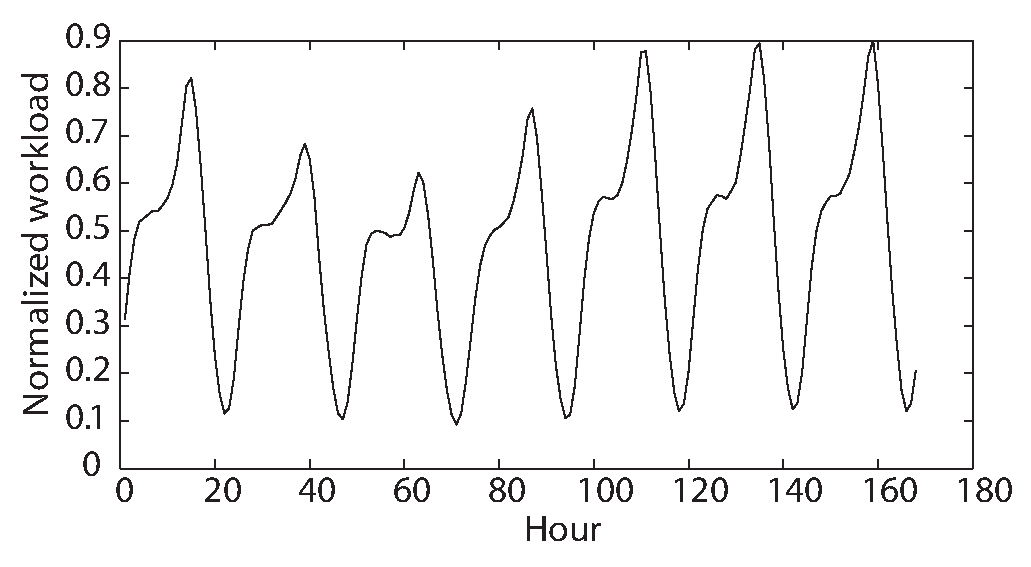
\includegraphics[width=\linewidth]{pics/workloadr.eps}
    \caption{Normalized workload}
    \label{fig:workloadr}
  \end{minipage}
  \hspace{0.5cm}
  \begin{minipage}[b]{0.5\linewidth}
    \centering
    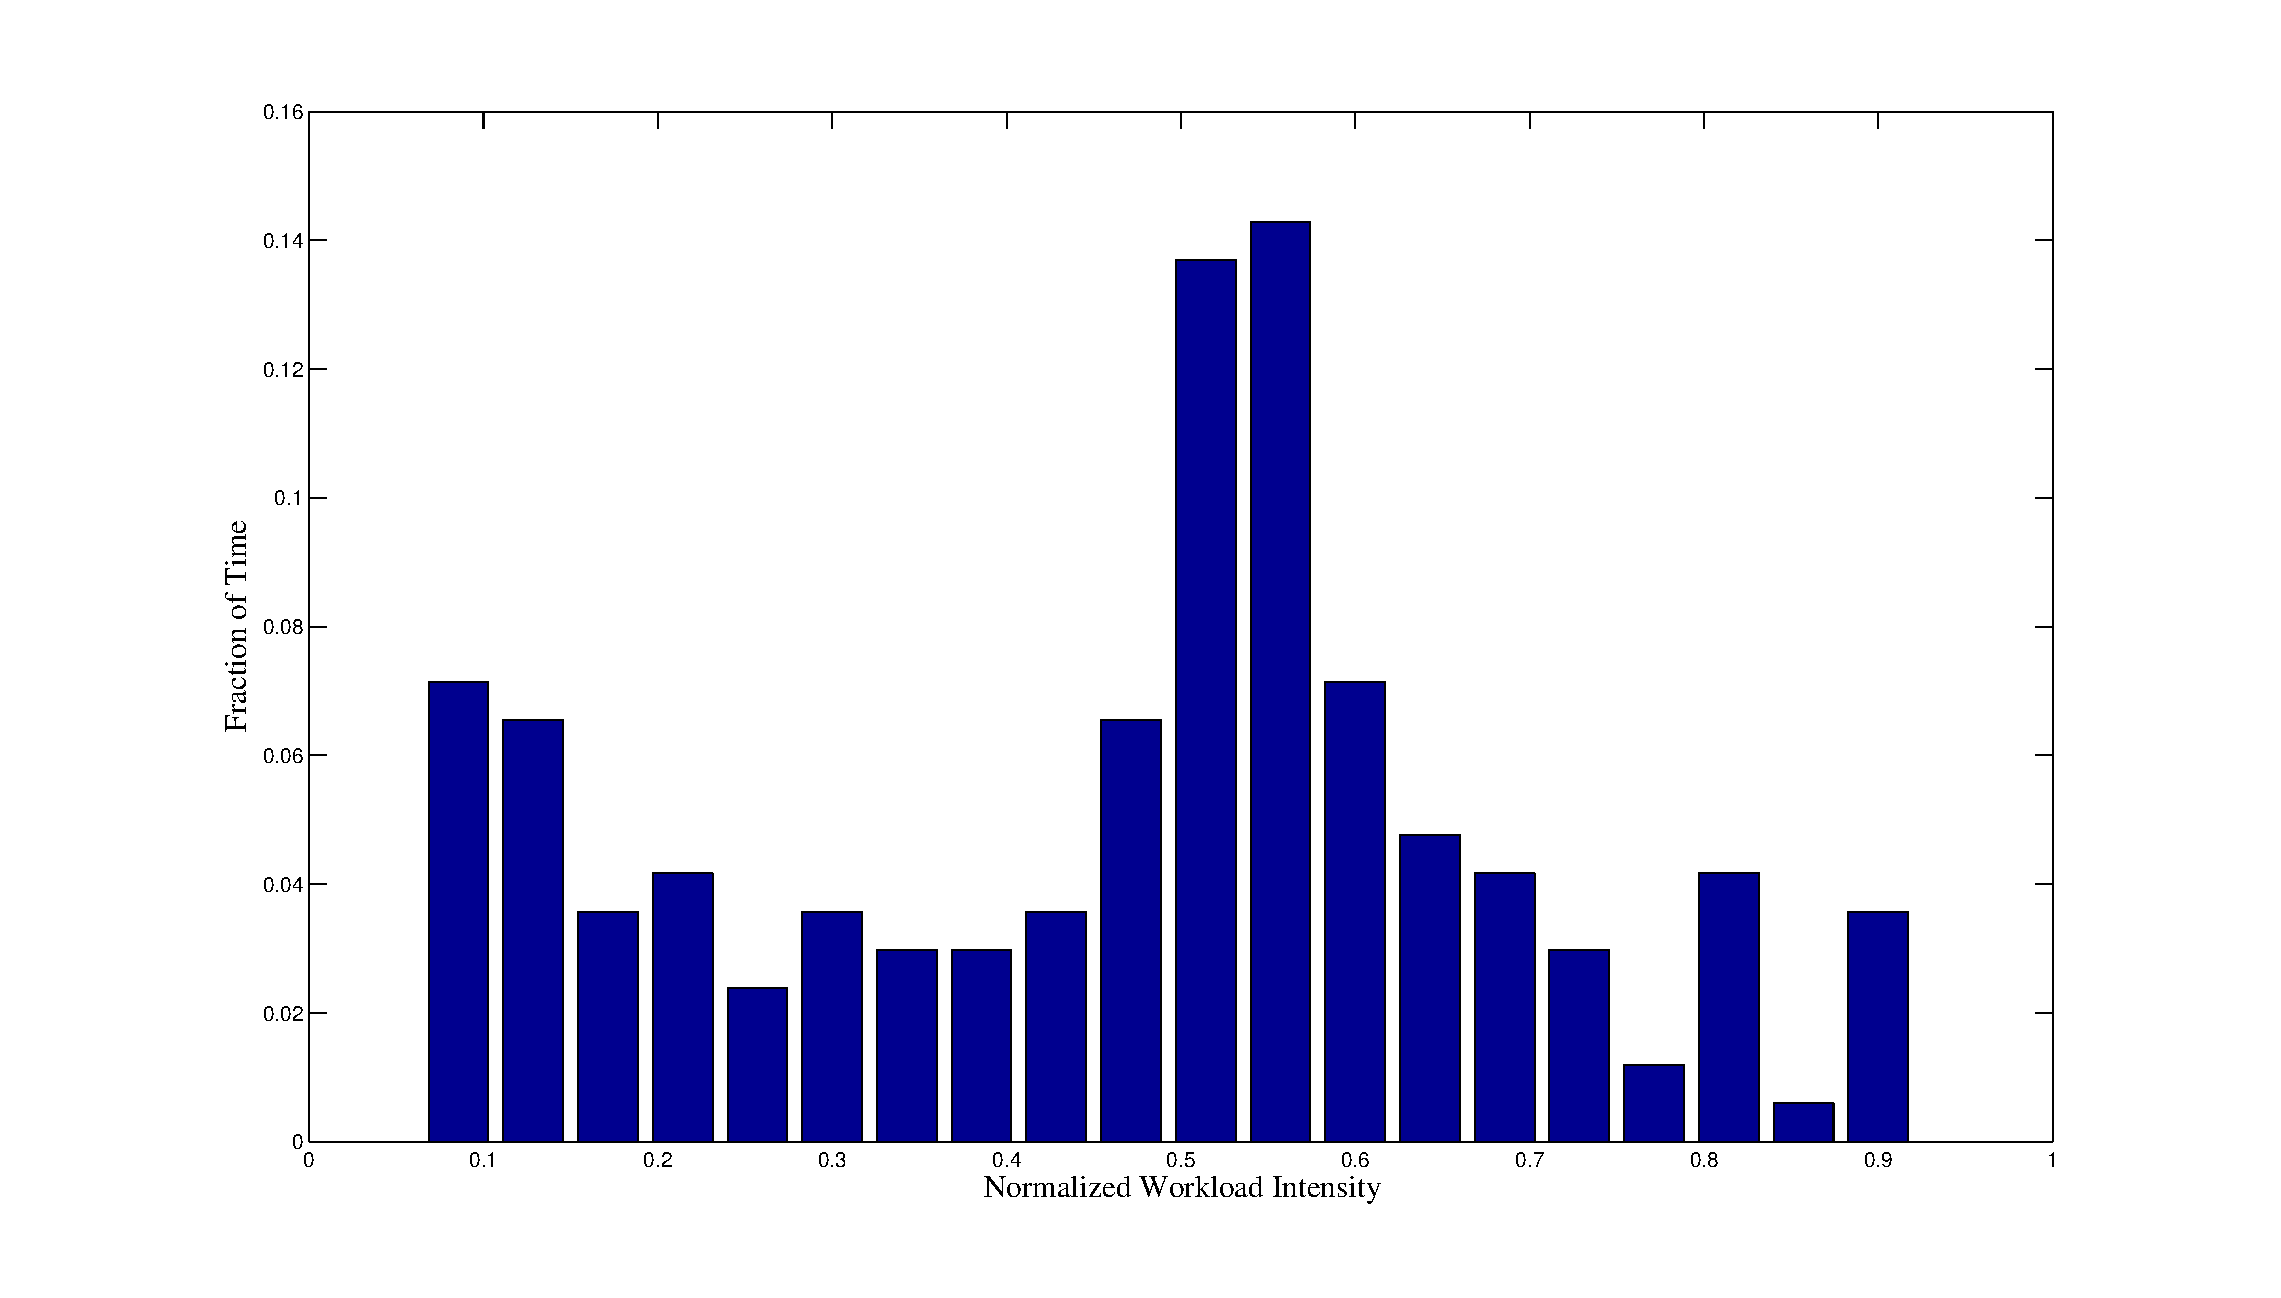
\includegraphics[width=\linewidth]{pics/workloadhist-new.eps}
    \caption{Workload intensity histogram}
    \label{fig:workloadhist}
  \end{minipage}
\end{figure}

\subsection{Electricity prices}
\label{subsec:prices} We selected $33$ different regions in the USA for which hourly electricity prices are available online. These regions belong to the following Independent System Operators (ISOs): NYISO, CAISO, MISO, ISO-NE and PJM. %To ease reproducibility of our results, the names for these locations as used in the online datasets are listed in Table~\ref{tab:locations}. 
We used the day-ahead prices for these locations, i.e., the electricity price negotiated for the same hour on the following day. In all the experiments for this thesis, we considered an operator with data centers at all 33 locations in our dataset. 

%\begin{table}
%\begin{center}
%\scalebox{0.7}
%{
%\begin{tabular}{|c|c|c|c|c|c|c|c|c|c|c|c|}
%\hline S. No. & Source & S. No. & Source & S. No. & Source & S. No. & Source & S. No. & Source & S. No. & Source \\
%\hline 1 & CAPITL & 7 & LONGIL & 13 & OH & 19 & MISO & 25 & WCMass & 31 & SEMass \\
%\hline 2 & CENTRL & 8 & MHKVL & 14 & PJM1 & 20 & Illinois & 26 & Boston & 32 & Vermont\\
%\hline 3 & DUNWOOD & 9 & MILLWD & 15 & WEST & 21 & Cinergy & 27 & CT & 33 & PJM2\\
%\cline{1-10} 4 & GENESE & 10 & NYC & 16 & PGAE & 22 & Michigan & 28 & Maine & \ & \ \\
%\cline{1-10} 5 & HQ & 11 & NORTH & 17 & SCE & 23 & Minnesota & 29 & NH  & \ & \ \\
%\cline{1-10} 6 & HUDVL & 12 & NPX & 18 & SDGE & 24 & First Energy & 30 & Rhode & \ & \ \\
%\hline
%\end{tabular}
%}
%\caption{Sources of electricity prices used in our work}
%\label{tab:locations}
%\end{center}
%\end{table}

%\begin{table}
%\begin{center}
%\begin{tabular}{ll}
%\hline Algorithm & Remarks \\
%\hline LI & Local optimal with idling \\
%LD & Local optimal with deactivation \\
%LS & Local optimal with selection \\
%LO & Local optimal without transition costs \\
%RED-BL & The global optimal solution for the planning window\\
%UNIFORM & Distribute workload equally over all data centers in all intervals \\
%%STATIC\_MIN & A single site data center operator \\ 
%\hline
%\end{tabular}
%\caption{Algorithms compared in our work}
%\label{tab:algos}
%\end{center}
%\end{table}

\subsection{Algorithms for Workload Distribution/Relocation}
\label{subsec:metrics} The workload relocation problem has the following dimensions based on which different algorithms may be formulated. 

\begin{itemize}
\item For a given interval, the strategy for distribution of workload amongst data centers.
\item For a given interval, the strategy for the state (on/off) of elastic load at a data center which has not been assigned any workload. In such cases, there is a trade-off between keeping the elastic load on (and incurring idling costs) and deactivating it (while incurring deactivation overhead and possibly activation overhead if it needs to be brought back online later in the planning window).
\item Over the planning window, does the algorithm report transition costs in the total electricity cost?
\end{itemize}

In this thesis, we report comparative results for six workload placement algorithms.%, listed in Table~\ref{tab:algos}. 
 The following list describes and differentiates these algorithms. The same comparison is also presented in tabular form in Table~\ref{tab:algosmatrix}.

\begin{itemize}
\item \textbf{RED-BL:} This is our proposed algorithm that determines the global optimal cost of electricity over a planning window while considering and reporting the transition costs. The choice of workload distribution as well as the state of elastic resources with no workload is governed by the optimal solution as determined by the CPLEX solver.
\item \textbf{Heuristic:} This is the heuristic algorithm that we proposed in Section~\ref{subsec:complexityheur}.
\item \textbf{UNIFORM:} This algorithm represents the choice of those operators that find an even loading of their data centers desirable. This algorithm does not deactivate elastic loads and hence does not incur transition costs.
\item \textbf{Greedy algorithms:} The originally proposed algorithm in~\cite{qureshi2009cutting} distributes workload to data centers such that, for each interval in the planning window, it makes a greedy assignment (in terms of current electricity price) of workload to data centers. Furthermore, this original algorithm keeps the elastic load at all data centers active in all intervals, incurring significant idling costs and hence is naturally disadvantaged against RED-BL. To have a fair comparison with the greedy workload distribution strategy, we use several variants of the original algorithm as well.
\begin{itemize}
\item \textbf{Local optimal with Idling (LI):} This is the originally proposed algorithm from~\cite{qureshi2009cutting}. It does not deactivate elastic load.
\item \textbf{Local optimal withOut transition costs (LO):} This variant of LI was proposed in~\cite{qureshi2009cutting}. It deactivates un-needed elastic load while ignoring the transition costs. This algorithm does not report transition costs in the total electricity cost of it's proposed workload mapping for the planning window. This algorithm is very useful because it defines the lower bound on electricity cost that any algorithm can ever achieve.
\item \textbf{Local optimal with Deactivation (LD):} This algorithm is similar to LO in all respects except that it also reports the activation/deactivation costs as part of the total cost of it's proposed solution. Unlike LO, it's results are practically relevant. It's total cost is less than (for all practical cases) LI, which makes it somewhat competitive to RED-BL.
\item \textbf{Local optimal with Selection (LS):} In cases where transition costs are high compared to idling costs it would be better to keep the elastic resources at a data center active and incur idling costs if it will be needed again after the lapse of a small number of intervals. LS is a variant of LD that is empowered with the ability to \textit{select} whether to deactivate unneeded elastic load at a data center or keep it idling. The cost of LS is never greater than that of LD.
\end{itemize}
\end{itemize}

\begin{table}
\begin{center}
\begin{tabular}{|c|c|}
\hline \multicolumn{2}{ |c| } {\bf{Workload mapping strategy}}\\
\hline LI, LD, LS, LO & Greedy \\
\hline RED-BL & Based on global optimal solution \\
\hline UNIFORM & Workload equally divided amongst all data centers \\
\hline \multicolumn{2}{|c|}\ \\
\multicolumn{2}{ |c| } {\bf{State of a data center in an interval when it has no workload}}\\
\hline LI & Active and idling \\
\hline LD, LO & Inactive \\
\hline LS & Either inactive or idling, whichever is cheaper \\
\hline RED-BL & Based on global optimal solution \\
\hline UNIFORM & Active \\
\hline \multicolumn{2}{|c|}\ \\
\multicolumn{2}{|c|}{\bf{Is transition cost reported in the total electricity cost reported?}}\\
\hline LI & N/A \\
\hline LD, LS & Yes \\
\hline LO & No \\
\hline RED-BL & Yes \\
\hline UNIFORM & N/A \\
\hline
\end{tabular}
\caption{A comparison of the algorithms studied in this thesis}
\label{tab:algosmatrix}
\end{center}
\end{table}


\section{Results}
 To evaluate the utility of workload relocation for electricity cost minimization, we
formulated seven different scenarios. For each scenario, we ran
seven experiments (one for each day's workload in our dataset) and report the average of the total electricity cost for each algorithm. Each experiment determines an operational plan for a planning window consisting of $24$ consecutive intervals, each with a duration of one-hour.

\begin{figure}
\centering
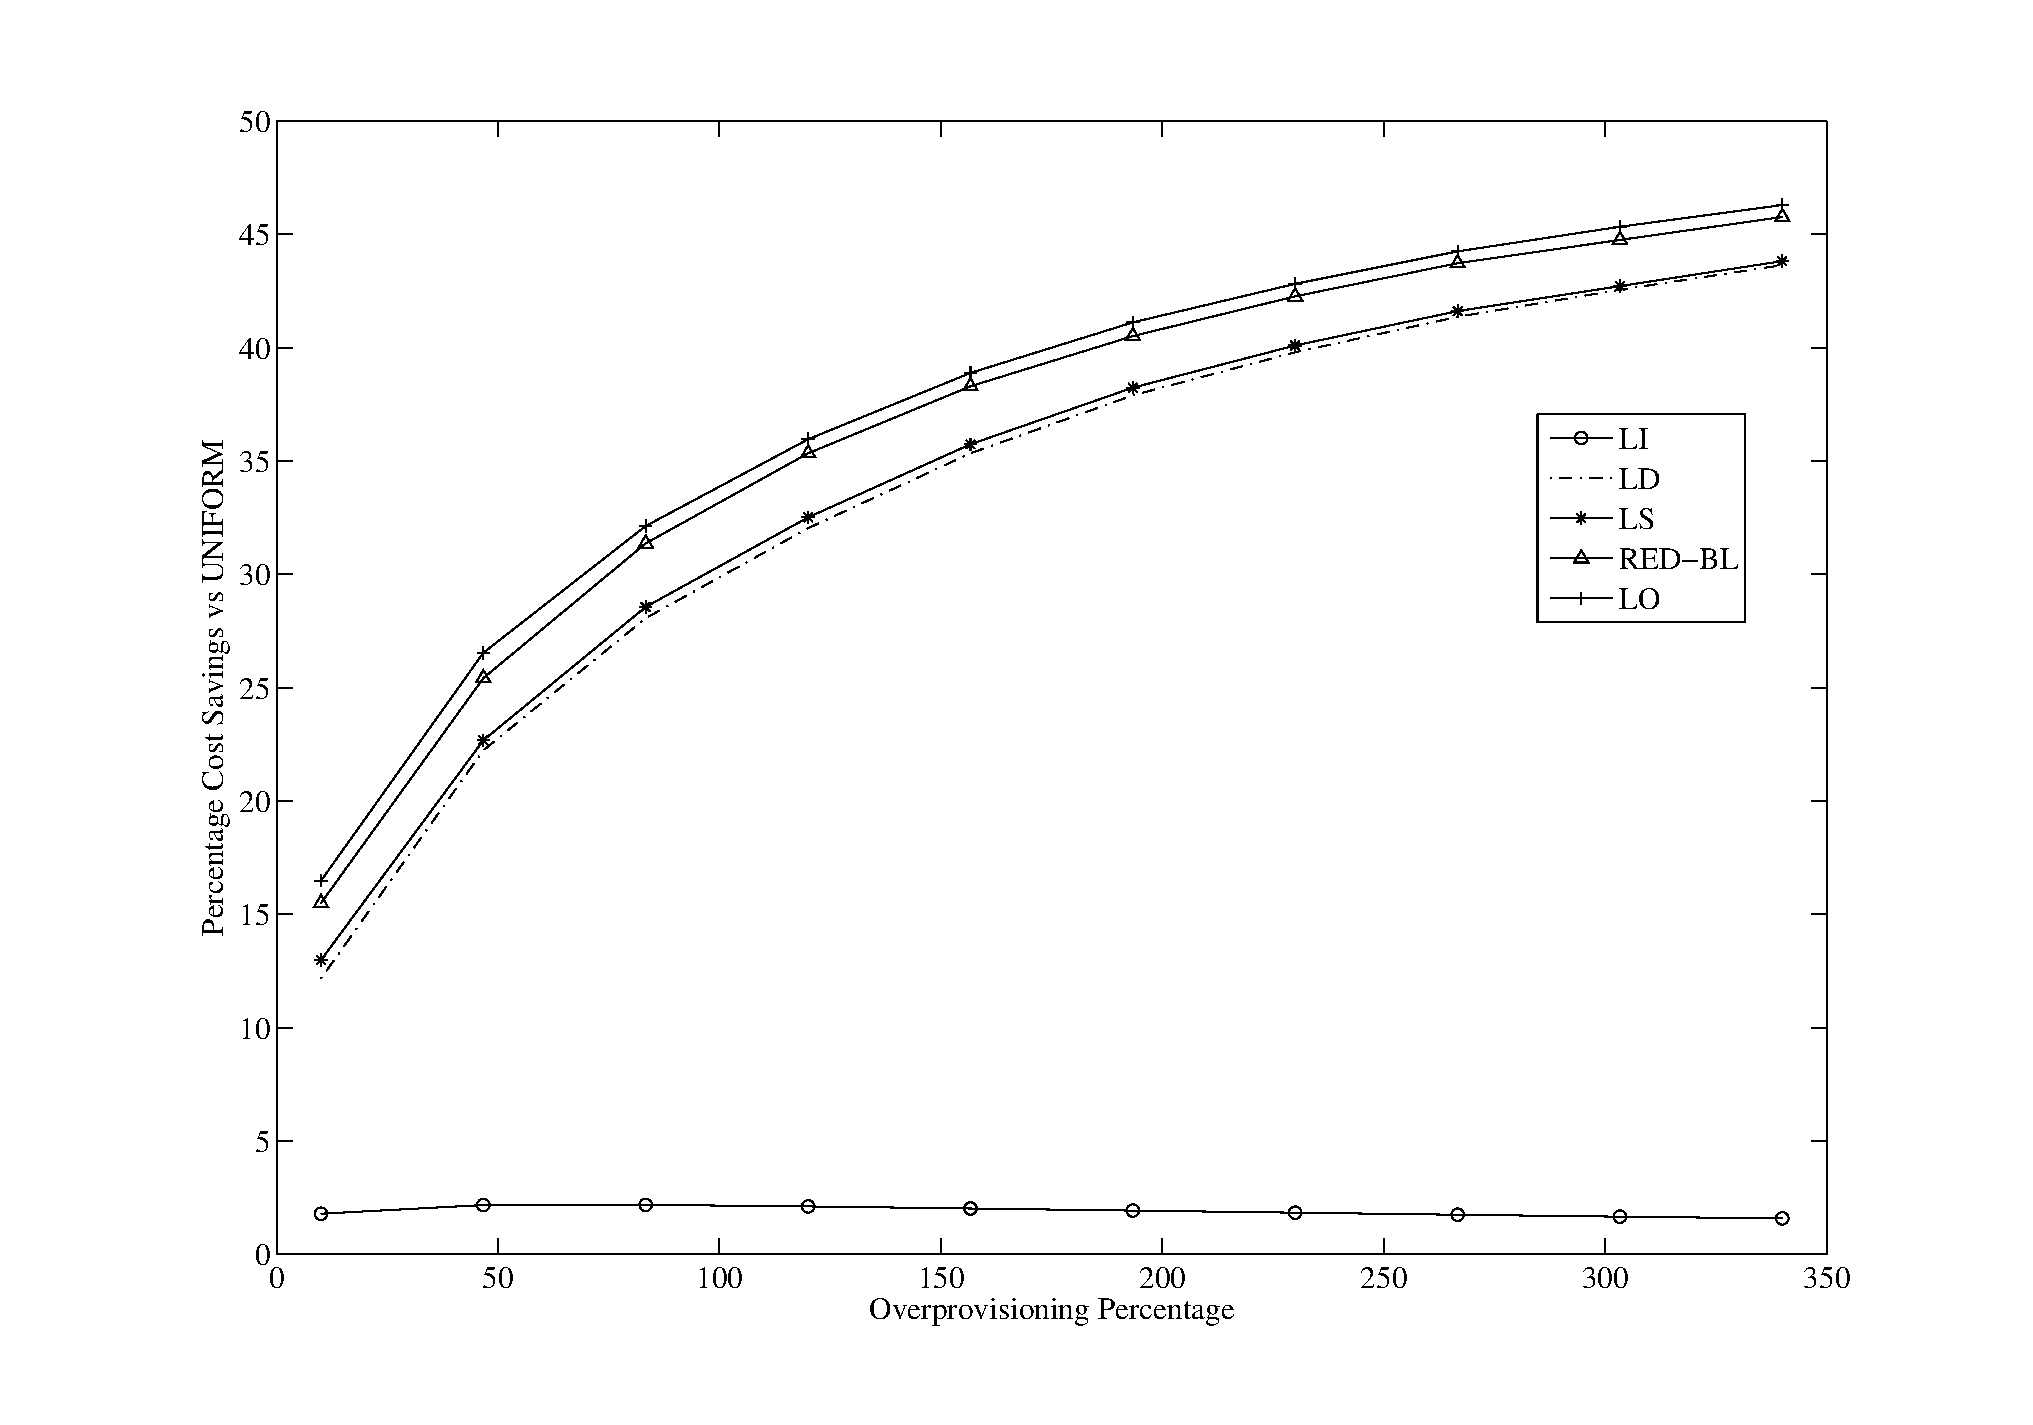
\includegraphics[width=\textwidth]{pics/s1vseqr.eps}
    \caption{Percentage savings with over-provisioning}
    \label{fig:s1r}
\end{figure}

\subsection{Sensitivity of electricity cost savings to extent of over-provisioning}In this scenario, we investigate the relationship of the amount of data center capacity over-provisioning with the electricity cost savings. As we increase the amount of over-provisioning, each individual data center's capacity would increase enabling more and more workload to be mapped to data centers at locations with cheaper electricity price.

With data centers at all
    $33$ locations in our dataset, we varied $c_i$ between $0.03$ and
    $0.12$ (in increments of $0.01$). This covers a variety of operators whose workload capacity ranges from just over expected peak workload to
almost $300\%$ over-provisioning.

We computed the total electricity cost for all algorithms while setting $f=\sigma=\delta=0.65$. The percentage savings in total electricity cost by various algorithms compared to UNIFORM are plotted against the data center capacity over-provisioning in Figure~\ref{fig:s1r}. We found that for the wide range of capacity over-provisioning that we considered, LI is able to do only slightly better than the naive UNIFORM algorithm (about 2\%). This is due to the significant idling costs incurred by LI under the experiment's conditions. For this reason, we have omitted LI from this plot.

The most competitive practical variants of LI, i.e., LS was 10.35\% off from the ideal lower bound (LO). Meanwhile, RED-BL solution is quite close the ideal lower bound (LO). The reason for greater savings with RED-BL compared to the greedy solutions (LS and LD) is that, the transition costs being significant, the former does fewer state transitions. In several intervals, RED-BL chooses data centers with relatively higher electricity price than the greedy solutions, but makes up for the higher computational cost by a reduction in the transition costs incurred.

\subsection{Sensitivity of electricity cost savings to magnitude of transition costs}
As the magnitude of transition costs relative to the state cost for an interval grows beyond a certain point, the benefits of deactivating elastic load at data centers would diminish. Accordingly, the electricity cost savings achievable by the workload relocation schemes would drop with increase in transition costs. In this scenario, we determine the percentage savings in total
    electricity cost for each algorithm, except
    STATIC\_MIN\footnote{STATIC\_MIN uses a static workload mapping so it is insensitive to variations in transition costs}, compared to UNIFORM, while varying the activation/deactivation overhead
    between $0$ and $1$, in increments of
    $0.1$. The lower bound on $\sigma$ (and $\delta$)
    implies the ideal condition of no transition overheads.
    We set the upper bound to $1$ so that the
    transition costs equal the cost of operating a data
    center at full load for an interval. A transition cost
    higher than this does not make sense as a workload relocation scheme would be better off keeping the elastic load at unloaded data centers idle. In this scenario,
    we kept $f=0.65$.

LI does not (de)activate unneeded elastic load and thus it's electricity cost is independent of the magnitude of transition costs. We observed taht it offered a saving of merely 1.74\% compared to UNIFORM. Figure~\ref{fig:s3r} shows the electricity cost savings for the other algorithms compared to UNIFORM. The LS and LD adaptations of the LI algorithm offer savings that scale almost linearly to the magnitude of transition costs. Both LS and LD also bring an average reduction in the elastic load's electricity cost sby a factor of $4$, compared to that of LI. RED-BL not only scales better than LS and LD but also achieves electricity cost saving that is fairly close (only $3\%$ higher, on average) than the ideal lower bound as reported by LO.


\begin{figure}[htbp]
  %\begin{minipage}[b]{0.5\linewidth}
    \centering
    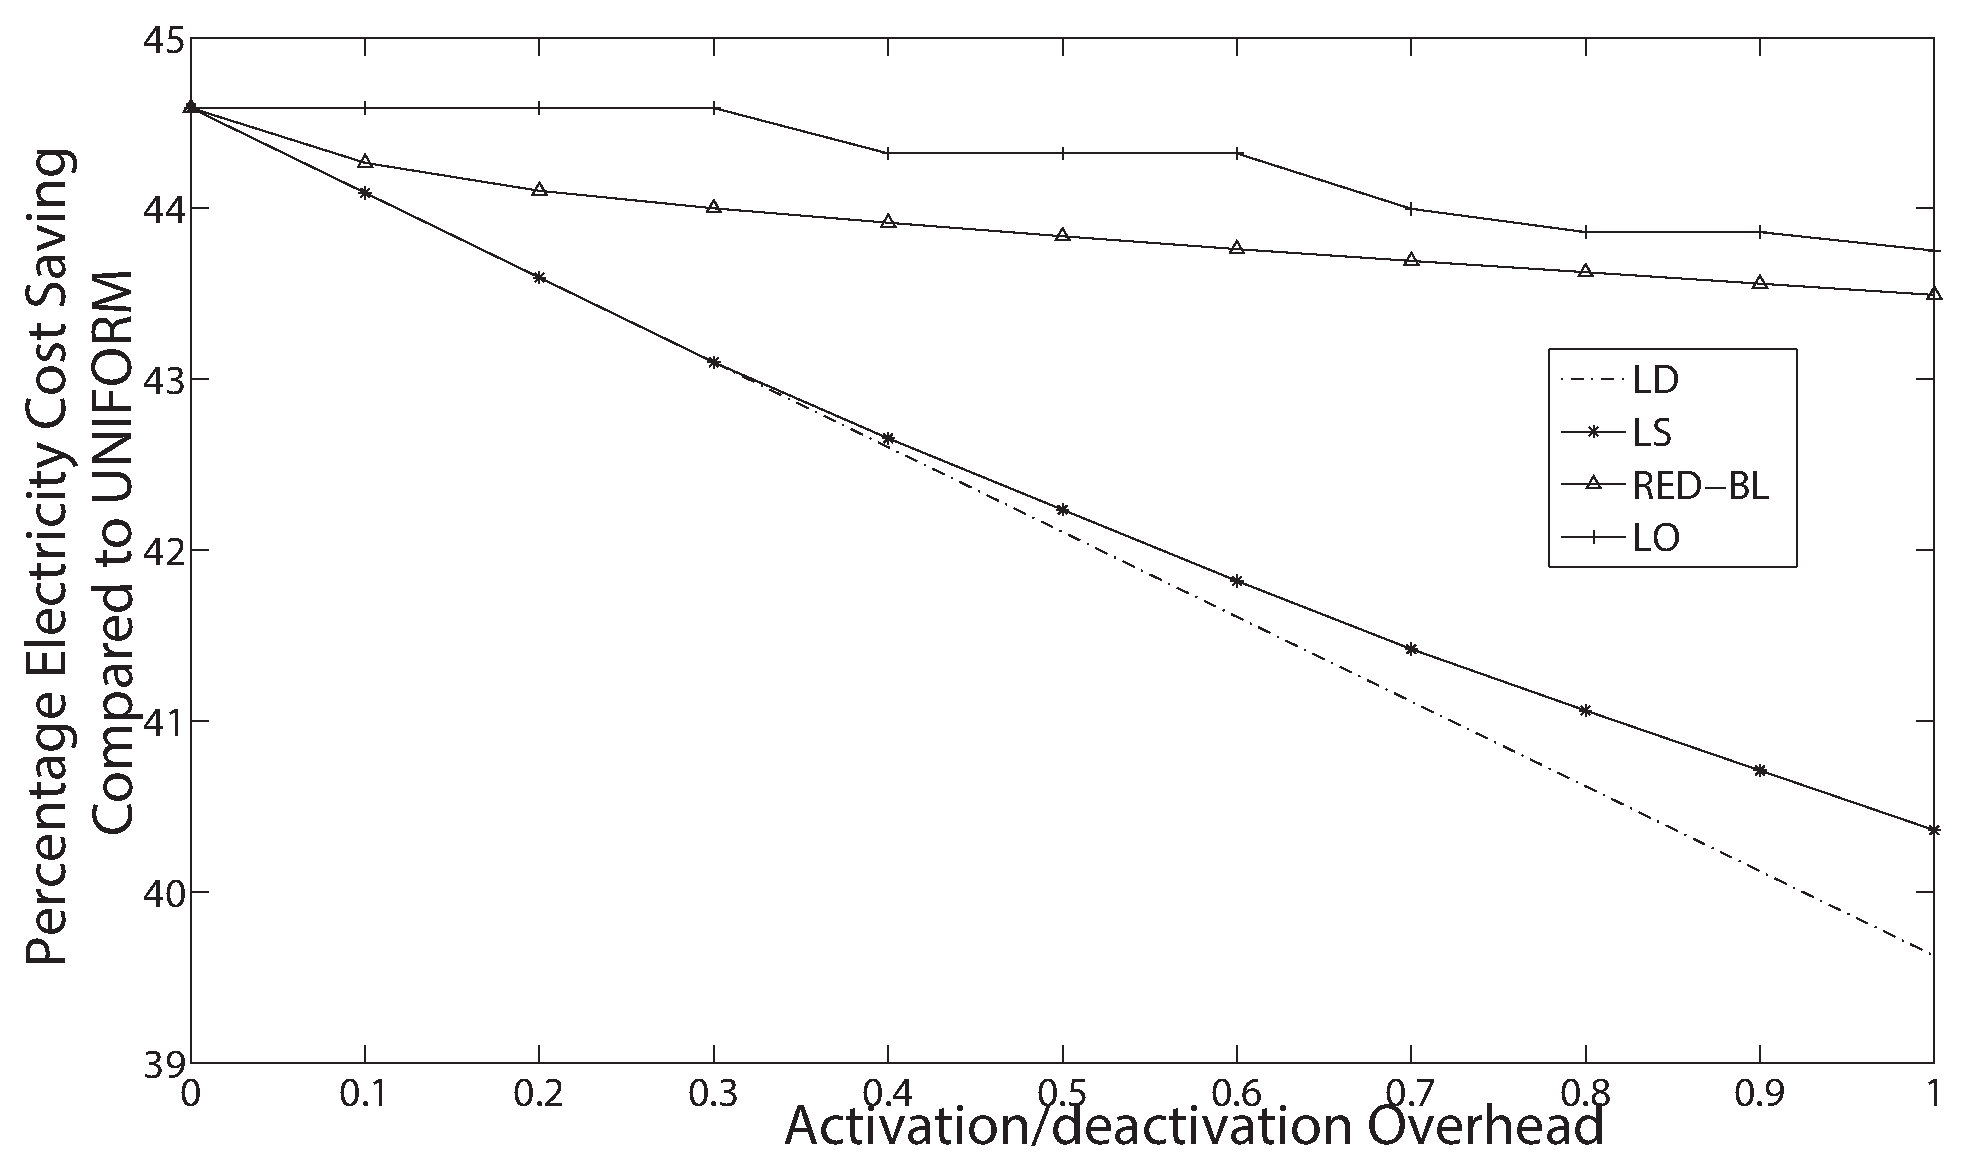
\includegraphics[width=1\linewidth]{pics/s3r.eps}
    \caption{Total cost vs transition overhead}
    \label{fig:s3r}
  %\end{minipage}
  %\hspace{0.5cm}
%  \begin{minipage}[b]{0.5\linewidth}
%    \centering
%    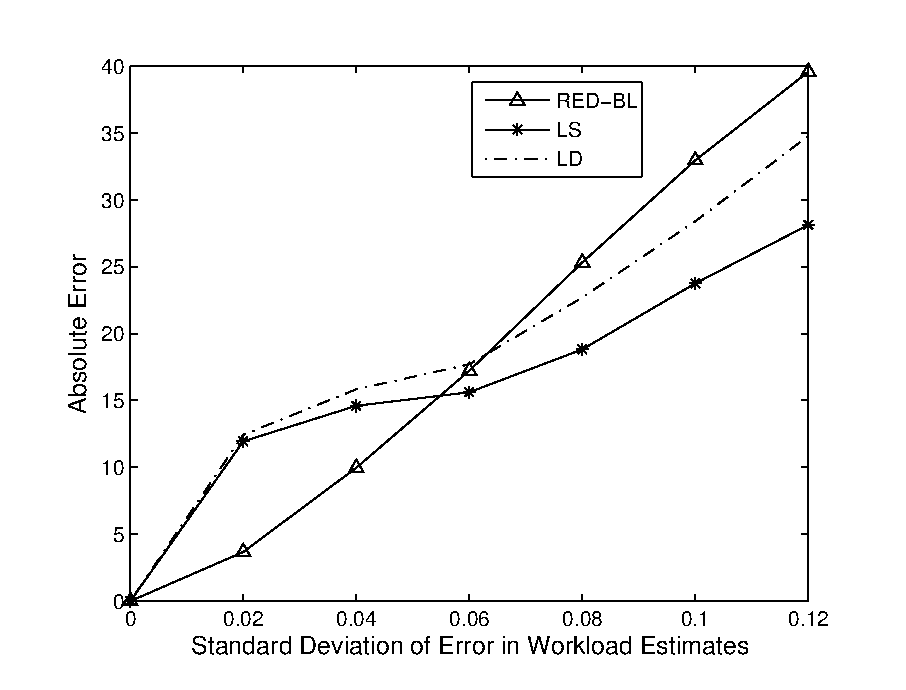
\includegraphics[width=1\linewidth]{pics/s4.eps}
%    \caption{Cost estimation error due to workload estimation error}
%    \label{fig:s4r}
%  \end{minipage}
\end{figure}

\subsection{Sensitivity of electricity cost savings to resource pruning granularity}
In this scenario, we investigate the potential benefits of deactivating the elastic load in a data centers in equal sized chunks instead of an all or nothing approach. The size of the portion of the elastic load in a data center that may be independently (de)activated may be deployment-dependent or operator-dependent. Possible choices of granularity may be a rack, a pod or one half of the elastic load etc. This granular deactivation can also be seen as throttling the equipment in a data center using facilities like processor frequency scaling. 

Granular (de)activation is expected to bring additional power savings. For instance, if the elastic load in a data center is operating at 10\% of it's capacity, then the remaining 90\% of the load is still consuming significant idling power. If we had the ability to power down half of the elastic load at a data center, we could cut idling energy cost significantly. 

The optimization problem formulation with $l$ granular (de)activation levels is given by:
 
\begin{align}
\text{minimize } \sum_{j=1}^{n} \sum_{i=1}^{m} c_i e_i^j(p_i^j \lambda(\frac{f}{l}+(1-f)\frac{x_i^j}{c_i}) + \frac{b_i^j \sigma}{l} + \frac{s_i^j \delta}{l})\notag
\end{align}
subject to:
\begin{align}
x_i^j \le c_i \hspace{6 pt} \forall i, \forall j \label{eq:gcapcon}\\
\sum_{i = 1}^{m} x_i^j = w^j \hspace{6 pt} \forall j \label{eq:gworkcon}\\
p_i^j, b_i^j, s_i^j \in \{0,1,...,l\} \hspace{6 pt} \forall i, \forall j \label{eq:ginteger1}\\
p_i^j \ge x_i^j*l/c_i \hspace{6 pt} \forall i, \forall j \label{eq:gp1}\\
b_i^j \ge p_i^j - p_i^{j-1} \hspace{6 pt} \forall i, 2 \le j \le n \label{eq:gbcon}\\
%\end{align}
%\begin{align}
s_i^j \ge p_i^{j-1} - p_i^j \hspace{6 pt} \forall i, 2 \le j \le n \label{eq:gscon}\\
b_i^0 = p_i^0, s_i^0 = 0 \hspace{6 pt} \forall i \label{eq:gbcon1}
\end{align}

There are three primary differences from the vanilla RED-BL formulation. The first difference is in the objective function, where the idling, bootup and shutdown costs depend on the number of granular units involved in the idling, bootup or shutdown process respectively. Since the computational cost component of power consumption only depends on the workload and is independent of the data center capacity, it is independent of the number of granular units being used at a data center during a given interval. The second difference is in the domain of $p_i^j$, $b_i^j$ and $s_i^j$ (see constraint~\ref{eq:ginteger1}). The third difference is in the constraint~\ref{eq:gp1}, which ensures that $p_i^j$ takes on an appropriate value from $0,1,...,l$.

\begin{figure}
    \centering
    \includegraphics[width=1\textwidth]{pics/s6.eps}
\caption{Cost saving vs (de)activation granularity}
\label{fig:granular-deactivation}
\end{figure}

In the current evaluation scenario, we explore how the RED-BL electricity cost savings scale with change in size of the unit of independent (de)activation. In Figure~\ref{fig:granular-deactivation}, we have plotted the percentage savings in electricity cost vs the granularity of data center's elastic load (de)activation. The savings are computed against the scenario where only the entire elastic load in the data center may be (de)activated as a whole. This baseline corresponds to a value of $l$ equal to one. Accordingly, in Figure~\ref{fig:granular-deactivation} we see no savings for that value of $l$. We also see that the ability to independently (de)activate half of a data center's elastic load provides around $2.5\%$ additional such savings on top of what the vanilla RED-BL can achieve. The electricity cost savings grow almost linearly when going to more granular size of independent (de)activation.

\subsection{Sliding window re-optimization}
With the exception of scenario 3, all of our simulation scenarios have been driven by error-free workload traces. The underpinning assumption to the corresponding results, therefore, is the availability of accurate workload estimates. We opine that this is not such a bad assumption given that the cumulative workload on the granularity of an hour changes slowly from one hour to the next and from one hour on a day to the same hour the next day. However, workload forecasting will have some error, however small it may be. 

In order to accommodate workload mis-estimation, we propose a sliding window-based algorithm that is somewhat similar to receding horizon control~\cite{rhc}. The algorithm is so called because it performs workload forecasts for a planning window and later slides the window by a constant offset before making another workload forecast, this time for intervals currently in the planning window. 

Our approach compensates for workload estimation errors on two (often) different time-scales. At an (often) longer timescale, the workload for the next $n$ intervals is forecast and a RED-BL plan is generated. This forecasting is repeated every $\gamma$ intervals, the \textit{window slide interval} parameter. The motivation is that at interval number 1, the workload forecast for interval number $gamma+k$ is expected to contain a greater amount of error than if the forecast for the same interval is done at interval $\gamma$, due to availability of more historical workload data at the later interval. This step of repeated forecasting and subsequent generation of a RED-BL plan is called \textit{global trajectory correction}. The basic idea behind this approach is that lowering of workload estimation error should bring the planned state trajectory closer to the optimal state trajectory (the one that results from perfect workload estimates). 

On a relatively shorter timescale, in each interval, our algorithm locally corrects for forecasting errors. The planned state for an interval may be \textit{infeasible} in the sense that it may be based on an under-estimation of workload and we might not have sufficient active data center capacity for the actual workload. Also, in case of over-estimation of workload, the originally planned state may be \textit{locally sub-optimal} as some data center resources would unnecessarily consume idling costs. This step that corrects for locally infeasible or sub-optimal states, considers only a single interval and, hence, is called \textit{local trajectory correction}. Upon entering an infeasible or locally sub-optimal planned state, we perform a local correction by finding a new state for the current interval. As shown in Figure~\ref{fig:traj-corr}, we start at the initial state $S_0$ and are scheduled to transition to state $\hat{S}_1$ at interval $1$. However, at interval $1$, we know the actual workload received and might discover that the planned state is locally infeasible or sub-optimal. To accommodate this, we transition to a locally better state $S_1$. At the end of interval $1$, we are scheduled to transition to state $\hat{S}_2$, and the process repeats. Since we only have accurate information about the workload for the present interval, the revision of the next state is always deferred to the next local trajectory correction step.

The local trajectory correction for interval $j$ is an optimization problem that attempts to minimize the electricity cost of the corrected state $S_j$ and the cost of transition between the planned state $\hat{S}_j$ and the corrected state. The mixed integer linear programming formulation for the local trajectory correction step for interval $j$ is as follows:
    
\begin{align}
\text{minimize } \sum_{i=1}^{m} c_i e_i^j(p_i^j \lambda(f+(1-f)\frac{x_i^j}{c_i}) + (b_i^j+\hat{b}_i^j) \sigma + (s_i^j+\hat{s}_i^j) \delta)
\end{align}
subject to:
\begin{align}
x_i^j \le c_i \hspace{6 pt} \forall i \label{eq:lcapcon}\\
\sum_{i = 1}^{m} x_i^j = w^j \hspace{6 pt} \label{eq:lworkcon}\\
p_i^j, b_i^j, s_i^j \in \{0,1\} \hspace{6 pt} \forall i \label{eq:linteger1}\\
p_i^j \ge x_i^j \hspace{6 pt} \forall i \label{eq:lp1}\\
b_i^j \ge p_i^j - \hat{p}_i^j \hspace{6 pt} \forall i \label{eq:lbcon}\\
s_i^j \ge \hat{p}_i^j - p_i^j \hspace{6 pt} \forall i \label{eq:lscon}\\
\hat{b}_i^j \ge \hat{p}_i^j - p_i^{j-1} \hspace{6 pt} \forall i \label{eq:lbcon1} \\
%\end{align}
%\begin{align}
\hat{s}_i^j \ge p_i^{j-1} - \hat{p}_i^j \hspace{6 pt} \forall i \label{eq:lscon1}
\end{align}

\begin{figure}
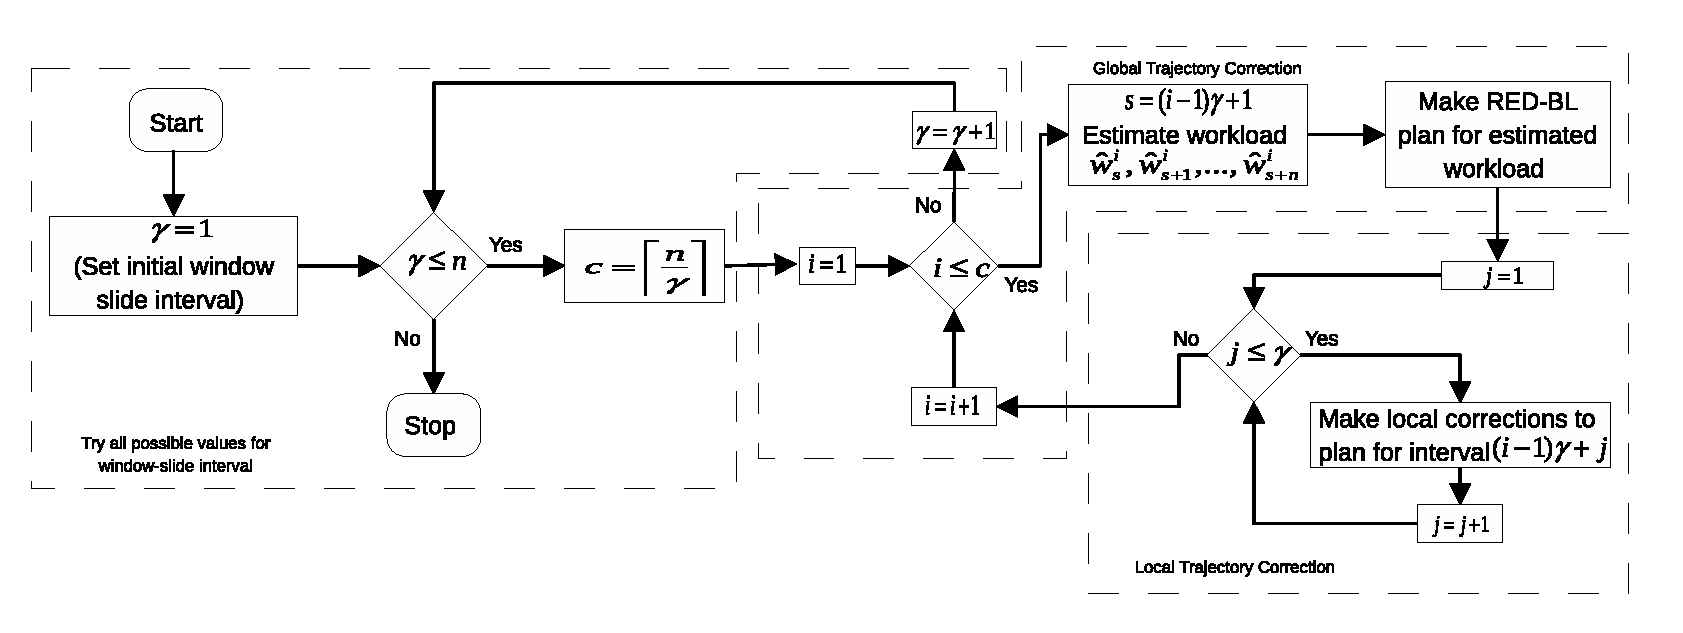
\includegraphics[width=1\linewidth]{pics/flowchart2.eps}
\caption{Flow of sliding window experiments}
\label{fig:flowchart}
\end{figure}

\begin{figure}[htbp]
  \begin{minipage}{0.45\textwidth}
    \centering
    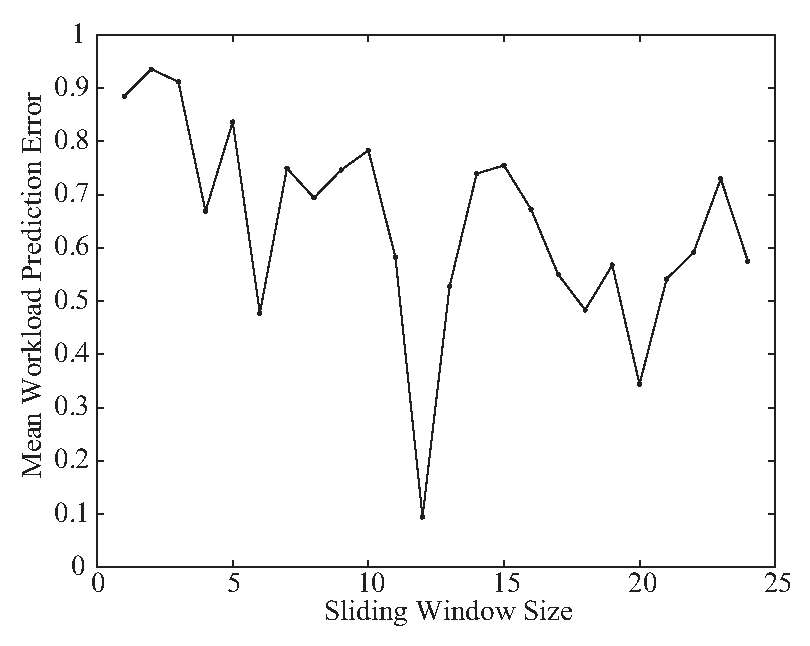
\includegraphics[width=0.8\textwidth]{pics/workload-pred-error-mean.eps}
    \caption{Mean absolute workload prediction error vs sliding window size}
    \label{fig:workload-pred-error-mean}
  \end{minipage}
  %\hspace{0.5cm}
  \begin{minipage}{0.45\textwidth}
    \centering         
    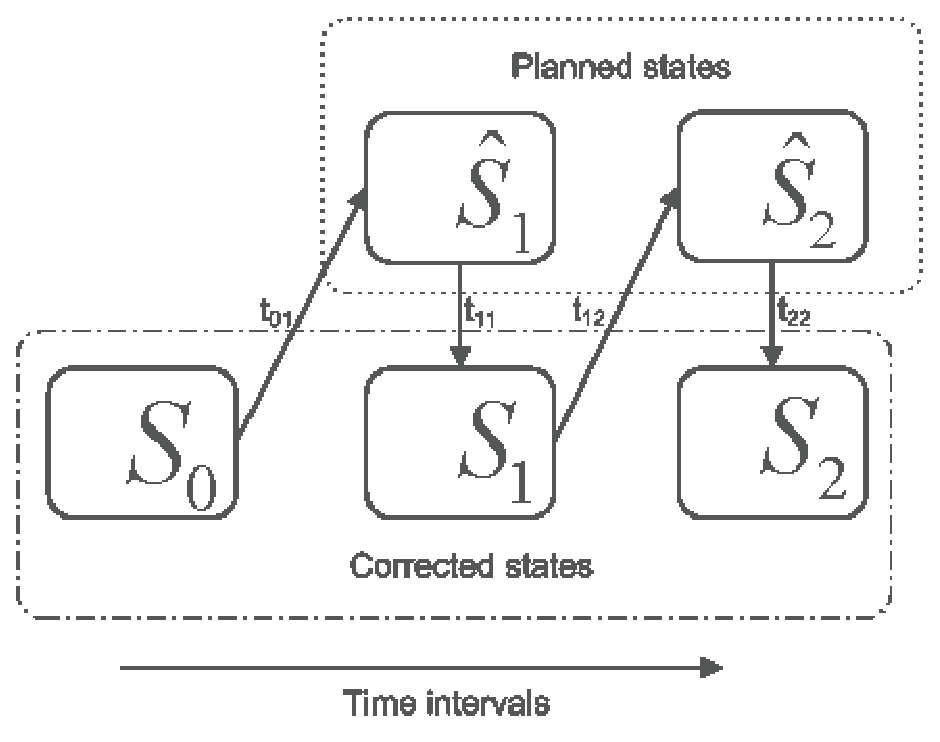
\includegraphics[width=0.8\textwidth]{pics/traj-corr.eps}
    \caption{Local trajectory correction technique for three consecutive intervals}
    \label{fig:traj-corr}
    \end{minipage}
\end{figure}

\begin{figure}
\centering
\includegraphics[width=0.5\linewidth]{pics/workload-pred-error-2.eps}
    \caption{Distribution of workload prediction error for sliding window size of 12 hours}
    \label{fig:workload-pred-error-dist}
    \end{figure}
    
    Given that the planning window size is $n$ intervals, the possible values for $\gamma$ are $1, 2, .., \gamma$. We experimented with all possible values for $\gamma$. Figure~\ref{fig:flowchart} shows the flow of our experiments. We first pick a value for the window sliding interval and estimate the workload for the next $n$-intervals and then invoke RED-BL. As an example, consider $\gamma=2$. We start by forecasting the workload for the first $n$-intervals, denoted by $\hat{W}_1^2 = [\hat{w}_{1,1}^2, \hat{w}_{2,1}^2, ..., \hat{w}_{n,1}^2]$. Here, $\hat{w}_{j,1}^2$, for instance, represents the workload forecast for interval $j$ during the first forecasting operation while the value of $\gamma$ is 2. For workload forecasting, we trained an ARMA(4, 4)~\cite{arma} model on a day's workload. Using $\hat{W}^2_1$ as the expected workload vector, we propose a RED-BL deployment plan for the first $n$-intervals. After the lapse of $\gamma$ intervals, i.e., at the start of the third interval (for $\gamma$ = 2), we forecast the workload for the next $n$ intervals, leveraging the additional information about the actual workload for the first two intervals which was not available in the first forecast step at $t=0$. This forecast is denoted by $\hat{W}_2^2 = [\hat{w}_{3,2}^2, \hat{w}_{4,2}^2, ..., \hat{w}_{n+2,2}^2]$. Then, we compute the RED-BL deployment plan for intervals $3, 4,..., n+2$ as the global trajectory correction step. Since the window sliding interval size is $\gamma$ and the number of intervals in our experiments is $n$, the number of times the window must slide, for a given value of $\gamma$ is $\lceil n/\gamma \rceil$. For $\gamma$ = 1, our scheme reduces to something resembling receding horizon control.
    

Having trained the model on the first day's data, we ran experiments for the last six days' workload in our dataset. We computed the average error of the daily electricity cost reported by these experiments compared to the total daily electricity cost for the same period with perfect workload estimates. The size of the planning window was set to 24 hours. 

The first set of results in this scenario is the percentage workload estimation error for various sliding window sizes. We see in Figure~\ref{fig:workload-pred-error-mean} that the mean absolute percentage prediction error is less than $1\%$. The minimum mean error is for a sliding window size of $12$ hours. For this sliding window size, the distribution of percentage workload estimation error is plotted in Figure~\ref{fig:workload-pred-error-dist}. Most of the workload estimates are quite close to error-free, while a few estimates are as much as 24$\%$ off. This low average error for $\gamma$ = 12 is expected due the nature of daily variations in the cumulative workload.

The difference of the electricity cost resulting from the use of the sliding window trajectory correction approach compared to the optimal solution with perfect workload knowledge is plotted in Figure~\ref{fig:s5r}. We see that the electricity cost achievable with RED-BL in a sliding window fashion is within 5-7$\%$ of the optimal cost achievable with perfect workload estimates. 

\begin{figure}[htbp]
    \centering
    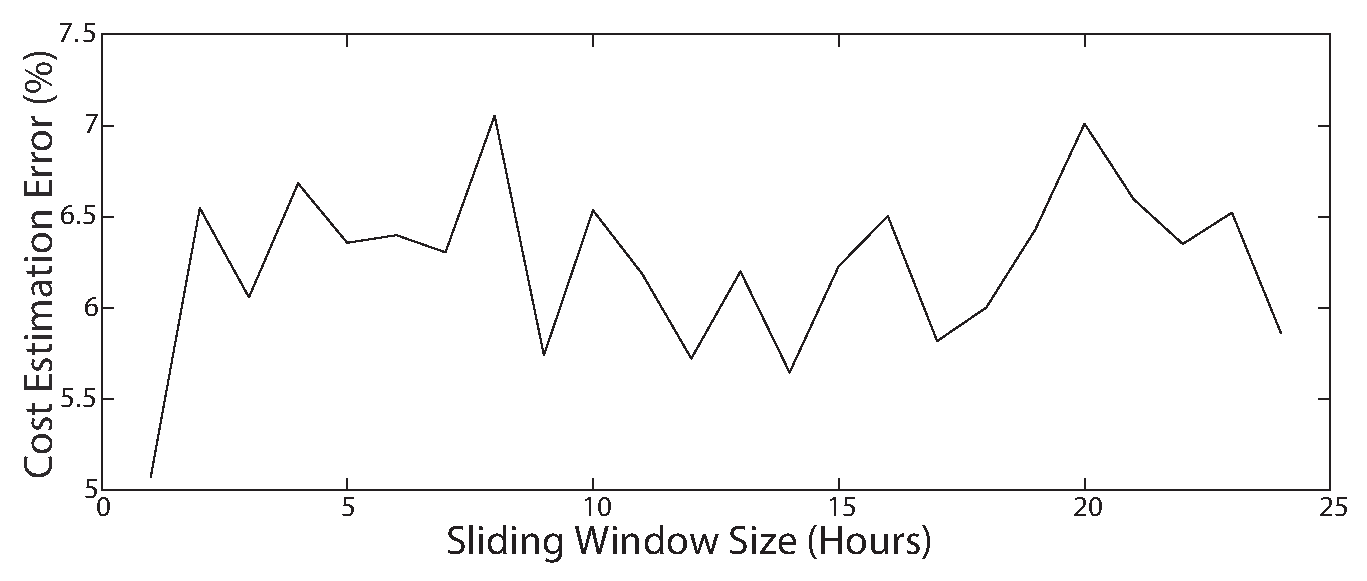
\includegraphics[width=1\textwidth]{pics/sw-cost-error-2.eps}
\caption{Percentage error of sliding window forecasts compared to global optimal with error-free workload}
\label{fig:s5r}
\end{figure}



\section{Sensitivity of electricity cost savings to the server idle-peak power ratio}
Chip manufacturers and computer vendors are striving to improve server energy propotional/efficient. It would be interesting to see how the electricity cost savings for RED-BL would improve as the server's idle to peak power ratio ($f$) drops. To this end, we conducted a set of experiments in which we kept all other parameters fixed while varying $f$ from 0 to 1.  Note that $f$=0 means that the servers are completely energy proportional, whereas $f$=1 means that the server power consumption is totally inelastic.

Figure~\ref{fig:fvar1} shows the variation of electricity cost savings as the value of $f$ is varied while the $b$/$s$ parameteres are kept at a low value of 0.01. In this setting, we wish to investigate if server energy proportionality improvement really matters if the bootup/shutdown costs were really low. Figure~\ref{fig:fvar1} shows that for an increase from $f$=0 to $f$=1, the global optimal solution over the planning window only spans an increase in average total electricity cost of 8.34\%. Also, a drop from the typical $f$=0.6 all the way to $f$=0 results in a 4.88\% drop in total electricity cost. It is noticeable that the bootup/shutdown overheads are really small and the idling fraction of electricity costs increases almost linearly with the value of $f$.
 
\begin{figure}
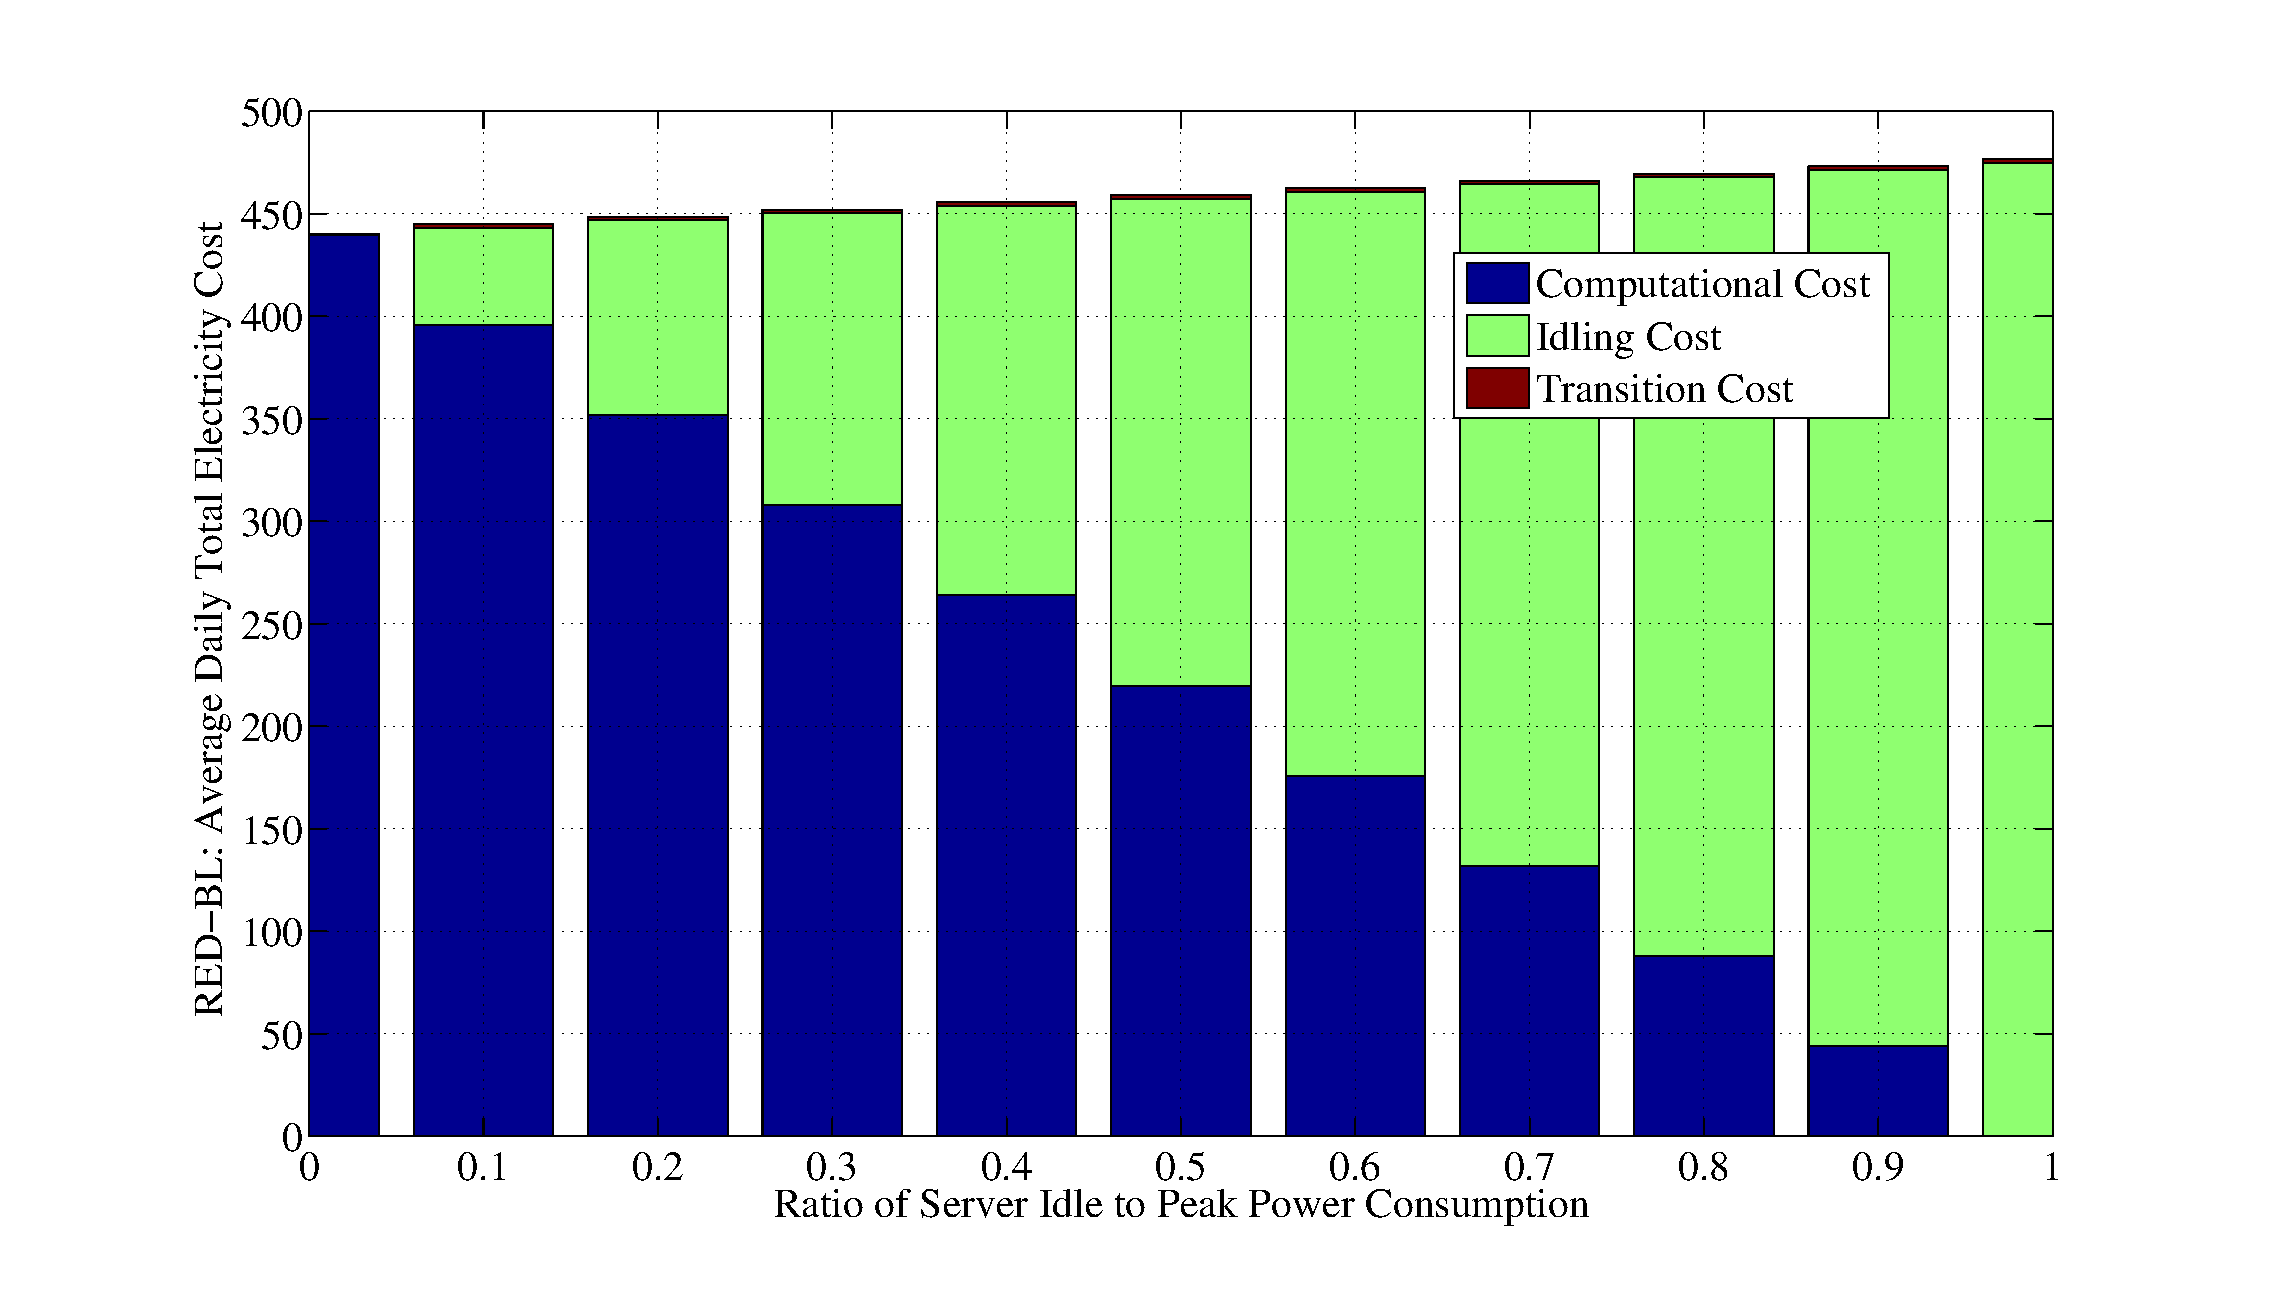
\includegraphics[width=1\textwidth]{pics/fvar-0.01bs.eps}
\caption{Average daily total electricity cost and it's components vs f, For bs = 0.01}
\label{fig:fvar1}
\end{figure}

\begin{figure}
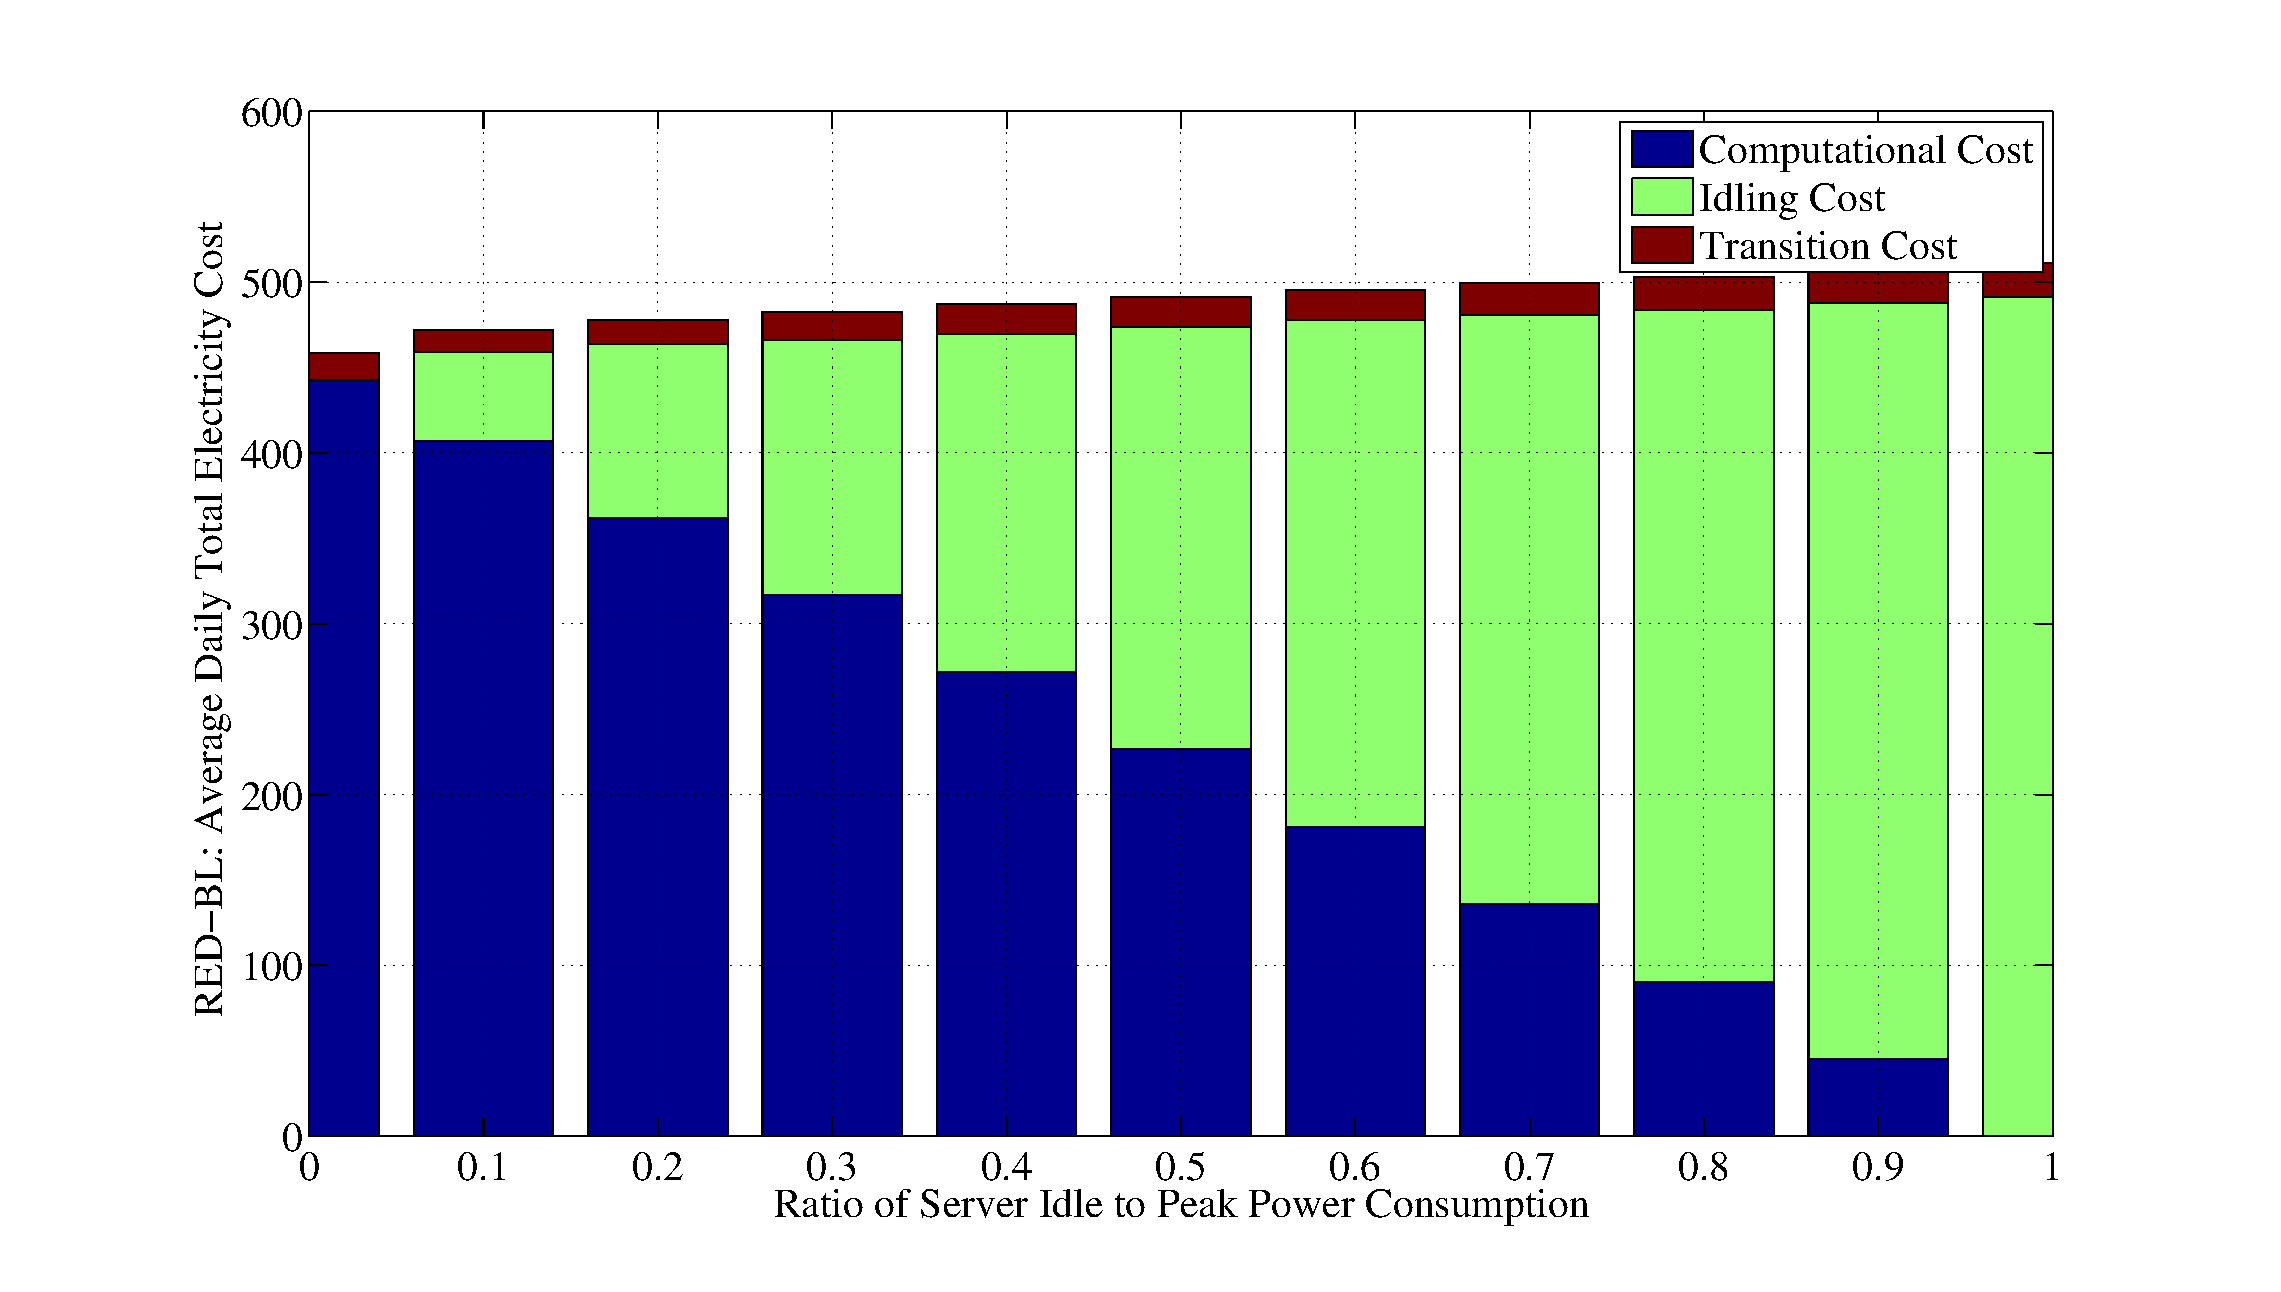
\includegraphics[width=1\textwidth]{pics/fvar-0.65bs.eps}
\caption{Average daily total electricity cost and it's components vs f, For bs = 0.65}
\label{fig:fvar2}
\end{figure}

Figure~\ref{fig:fvar2} shows the same results for $b$/$s$=0.65. In this case, an increase from $f$=0 to $f$=1 spans an 11.44\% increase in average daily total electricity costs. Also, as $f$ drops from the typical $f$=0.65 all the way to $f$=0, the total electricity cost of the global optimal solution over the planning window drops by 7.42\%. Since the bootup/shutdown overhead is significant in this case, for all values of $f$, the total electricity cost of the global optimal solution over the planning window is characterized by an almost fixed contribution from bootup/shutdown, while the idling fraction increase almost linearly.

\section{Performance of the heuristic algorithm}
Figure~\ref{fig:heur1perf} shows the performance of our heuristic algorithm compared to the optimal solution of the problem for various values of the (de)activation overhead parameters. For each value of the $b$/$s$ parameters, we have plotted the average error over the seven days in our workload dataset (the curve) as well as the minimum and maximum error for any given day (the vertical bars). The performance of the heuristic is the worst for $b$/$s$ = 0, because the heuristic avoids bootup/shutdown which has zero cost for $b$/$s$ = 0. For other small values of $b$/$s$ also, the bootup/shutdown overhead is not significant and by avoiding it, our heuristic fares relatively poorly compared to the optimal solution. As the value of $b$/$s$ increases, our heuristic's error compared to the optimal solution drops until it starts a slight rise. The rising trend in the heuristic's performance for relatively high values of $b$/$s$ is because in this regime, it may often be better to allow idling of some data centers instead of a bootup at the intervals defined by $p_1$ and shutdown at those defined by $p_2$. We observed similar trends for other values of $f$ as well, when $b$/$s$ is varied from 0 to 1.

\begin{figure}
\includegraphics[width=1\linewidth]{pics/rb-heur1error.eps}
\caption{The minimum, maximum and average percentage difference between the cost of our heuristic and RED-BL}
\label{fig:heur1perf}
\end{figure}

\section{Discussion}
In this chapter, we have instantiated the generalized problem formulation of joint workload relocation and resource pruning to optimize electricity costs for geo-diverse data centers. The generalized formulation performs a state trajectory optimization and in case of geo-diverse data centers, the network state consists of a combination of discrete as well as continuous variables. 

Our formulation determines a deployment configuration plan that is optimal over a planning window consisting of several intervals in the form of bootup/shutdown times for each data center as well as the workload to be mapped to each data center for all intervals in the planning window. Discrete optimization problems such as ours are difficult to solve exactly because of their computational complexity. However, using the CPLEX solver we were able to compute the optimal plans for planning windows consisting of 24 one-hour intervals within a few seconds. 

Our problem formulation involves several parameters whose values are expected to vary over time (for instance, the value of idle to peak power consumption ratio is expected to improve as chip and server energy proportionality improves), from one operator to another (for instance, the over provisioning ratio) and from application to application (for instance, the value of the transition cost). With so many parameters, each with many possible values, it is not possible to exhaustively test RED-BL. However, in such a case, it suffices to know the sensitivity of electricity cost savings to the variation in each parameter, while all others are held at some reasonable default values. We performed a series of such experiments for each parameter and reported the results.

Since RED-BL devises a deployment plan for a planning window based on workload forecasts, which may be somewhat erroneous, in a practical setting, RED-BL plans must be revised periodically to bring the system closer to an optimal state. For this purpose, we proposed a sliding-window re-optimization procedure and evaluated it's performance.

We used workload datasets from three live Internet applications. While the number of applications is quite small for a large geo-diverse data center operator, the statistical characteristics of the dataset are reasonably representative of such a scenario. We also used real electricity prices from 33 locations in the US that were publicly available.

While we find that RED-BL finds a useful application in electricity cost optimization of geo-diverse data centers, our thesis is not the final word on this problem. Several avenues of further exploration are yet to be explored. We have listed some future work in Chapter~\ref{chap:conclusions}.
\chapter{Case Study II: Cellular Networks}
\label{chap:casestudy2}
\section{Instantiating the generalized optimization formulation} Derive the objective function and constraints. Clearly outline the assumptions that we've made about the geo-diverse data centers.

\section{Experimental setup} 

\section{Results}
\subsection{Sensitivity of electricity cost savings to the duration of an optimization interval} We may optimize at different frequencies, such as once an hour or twice an hour. In this section, we study the sensitivity of electricity cost savings to the frequency of re-optimization
\subsection{Sensitivity of electricity cost savings to the resource pruning granularity} We may have two states for a BTS: (i) 6+6+6, (ii) 3+3+3. Or, we may have three states: (i) 6+6+6, (ii) 4+4+4, and (iii) 2+2+2. How do the two-state and three-state resource pruning granularity settings comapre in terms of electricity cost savings? 
\subsection{Sensitivity of electricity cost savings to the margin of state-change damping} Suppose that we are using a two-state resource pruning model. If $t_{max}$ is the call capacity of a 6+6+6 site, then the call capacity of the half-pruned site is $t_{max}/2$. If we deactivate TRXs immediately when the instantaneous call volume reaches $t_{max}/2$, we are likely to have many transitions due to short-term variations in call volume. We, therefore, wait until the instantaneous call volume is $t_{max}/2 - \epsilon$ before we switch to a $3+3+3$ configuration. The value of $\epsilon$ is a configurable parameter which can take a value from $0$ (very aggressive, lots of transients, perhaps more savings) to $t_{max}/2$ (very conservative, no transients, no savings either). How do the electricity cost savings vary with the value of $\epsilon$.

\section{Discussion}
\chapter{Conclusions and future work}
\label{chap:conclusions} Geo-diverse data centers and cellular networks are quite similar in some respects and hence may be abstractly represented as a set of resources. Each of these resources is constrained by the maximum amount of workload it can handle. Furthermore, for both cellular networks and geo-diverse data centers, the instantaneous power consumption for the resources is similar, i.e., an affine function of the amount of workload they handle. The no-load power consumption for the resources in these networks is a large fraction of the full-load power consumption. 

The workload is quite variable, and the network must be dimensioned according to peak workload demand. However, the workload peaks for only a short duration and drops to a much lower trough. Thus, these networks are energy inefficient and their electricity cost is quite high. One way to improve the energy efficiency and save electricity costs is to scale the networks resources in response to workload variations.

We represent the status (on or off) of network resources and the workload mapped to them as a network state. Using this representation, we model the energy efficiency improvement problem as an optimal state trajectory problem, which we call Relocate Energy Demand to Better Locations (RED-BL). We used workload traces collected from real networks and real electricity costs to assess the utility of RED-BL. In doing so, we have made the following contributions:
\begin{itemize}
\item We identified abstractions for a generic power consumption model applicable to two different networks: geo-diverse data centers and cellular networks. Our model represents these networks as a set of resources that have an associated workload handling capacity. When a resource handles workload, it consumes some power according to a power consumption function. 
\item The aggregate mapping of workload to resources may be viewed as a network state. We accordingly model the electricity cost minimization problem in networks as a multi-interval optimal state trajectory problem.
\item We provide a mathematical optimization formulation for the optimal state trajectory problem. The formulation is parameterized and abstract for broad applicability. We modeled state transition costs as being a fraction of the cost of a state in a single interval.
\item We apply the mathematical optimization problem to geo-diverse data centers as well as cellular networks with the following contrasts:
	\begin{itemize}
	\item The optimal mapping of workload to resources is a discrete optimization problem. The workload capacity of a single resource is quite large in case of geo-diverse data centers, hence any fraction of workload mapped to a resource is likely to be quite close to a whole number of client requests. If this is not the case, the number of client requests mapped to a resource may be rounded to the nearest integer. The difference in power consumption resulting from this rounding is expected to be quite small. Hence, the optimal mapping of workload to resources, which is a discrete optimization problem may be relaxed to a fractional problem without much error in case of geo-diverse data centers. In cellular networks, on the other hand, the number of workload units being handled simultaneously by a single resource is much smaller. Thus, a fractional mapping of workload to resources in a cellular network may represent a call being handled by multiple BTSs simultaneously, which does not make sense. Hence, a fractional relaxation to the optimization problem is not possible in case of cellular networks.
	\item A call may only be handled by a restricted set of nearby BTSs. In contrast, in a geo-diverse data center setting, it is common for applications to be replicated across data centers and in such cases, a client request may be handled at any data center.
	\item Geo-diverse data centers are so far apart that geographic diversity in electricity prices is quite apparent. Meanwhile, BTSs in cellular networks are not too distant and geographic diversity in electricity prices is not present.
	\item The transition costs in geo-diverse data centers are expected to be significant. However, in cellular networks, the electricity cost impact of resource activation and deactivation is negligible.
	\end{itemize}
\item We show that the electricity cost minimization problem is NP-Complete in both geo-diverse data center and cellular network scenarios and provide heuristic algorithms for solution of the problem in each of these networks. We were also able to solve reasonably sized problems for both network types.
\item We studied the sensitivity of the state trajectory problem to variations in the parameter values such as the magnitude of transition costs relative to the cost of a state in a single interval.
\end{itemize}

\section{Scope of our work} Like all research work, our work's scope is not unlimited. To the best of our knowledge, the following list covers the scope of our work:
\begin{itemize}
\item We only considered resource activation and deactivation costs as the source of transition costs. Data replication costs in geo-diverse data centers have not been evaluated because of (to the best of our knowledge) lack of models in the literature. Coming up with a general model for this cost is beyond the scope of this thesis.
\item For geo-diverse data centers, we have experimented with day ahead electricity prices for the US market. 
\item RED-BL computes the hourly traffic volume to be mapped to each data center. It does not provide a mapping of this workload to individual servers within the data center. This is a complementary research problem, which is presently receiving significant research attention.
\item In case of cellular networks, the ability to handle greater traffic volume through the half-rate codecs has not been considered.
\end{itemize}

\section{Future work} Some of the avenues for future inquiry related to our work are:

\begin{itemize}
\item Study the inter-data center traffic to examine if there is a relationship between the volume of such traffic with the number/nature of client requests, duration of the interval for which data volume is measured, or some other variables. This may help build a model for the expensive inter-data center traffic. Such a model may be integrated with RED-BL to have a more elaborate optimization framework that is sensitive to the potential increase in inter-data center traffic due to data center elastic resource (de)activation.
\item Replication of data stores across data centers requires some overhead traffic. An empirical study could be performed to build a model for such traffic in a few representative scenarios such as news websites, social networking sites, micro-blogging etc. Our work saves electricity cost by turning off elastic resources. This may mean taking the application data stores offline. When the elastic resources come back online, they would need to bring their data stores in sync with the rest of the data centers. The results of the aforementioned empirical study could be used to predict the volume of traffic that would be generated during this re-synchronization event.
\item The deployment of a small-scale GSM testbed using open source GSM software could be done to validate the results of our simulation study.
\item RED-BL may be applied to other networks such as generation resource scheduling in smart grids or packet switching networks.
\end{itemize}


\appendix
\bibliographystyle{ieeetr}
\bibliography{ref}

\end{document}

